\documentclass[12pt,a4paper,oneside]{report}             % Single-side
%\documentclass[11pt,a4paper,twoside,openright]{report}  % Duplex

\input{content/packages}

%--------------------------------------------------------------------------------------
% Language configuration -- choose one
%--------------------------------------------------------------------------------------
\input{content/thesis-hu}  % Beállítások magyar nyelvű dolgozathoz

%--------------------------------------------------------------------------------------
% Main variables
%--------------------------------------------------------------------------------------



% Szak alapkepzes vagy mesteri
\newcommand{\szakHU}{SZOFTVERFEJLESZTÉS SZAK}
\newcommand{\szakRO}{SPECIALIZAREA DEZVOLTAREA APLICAȚIILOR SOFTWARE}
\newcommand{\szakEN}{SOFTWARE ENGINEERING SPECIALIZATION} 


\newcommand{\dolgozattipusHU}{DIPLOMADOLGOZAT} 
\newcommand{\dolgozattipusRO}{LUCRARE DE DIPLOM\v A} 
\newcommand{\dolgozattipusEN}{BACHELOR THESIS} 

\newcommand{\szerzo}{Suciu Aksza}
\newcommand{\temavezetoA}{Dr. Buza Krisztián} 


\newcommand{\temavezetoAfokozat}{Egyetemi docens}
\newcommand{\temavezetoAfokozatRo}{Lector universitar}
\newcommand{\temavezetoAfokozatEn}{Lecturer}
\newcommand{\temavezetoB}{} 
\newcommand{\cimHu}{Echo: AI-alapú nyelvtanuló alkalmazás fejlesztése és oktatási célú értékelése}
\newcommand{\cimRO}{Echo: Development and Educational Evaluation of an AI-Based Language Learning Application}
\newcommand{\cimEN}{Echo: Dezvoltarea și evaluarea educațională a unei aplicații de învățare a limbilor stăine bazate pe inteligență artificială}
\newcommand{\ev}{2026}

\input{content/preamble.tex}




%--------------------------------------------------------------------------------------
% Table of contents and the main text
%--------------------------------------------------------------------------------------
\begin{document}
	
% CIMOLDALAK
%~~~~~~~~~~~~~~~~~~~~~~~~~~~~~~~~~~~~~~~~~~~~~~~~~~~~~~~~~~~~~~~~~~~~~~~~~~~~~~~~~~~~~~
	\include{content/titlepage}
	%--------------------------------------------------------------------------------------
%	The title page RO
%--------------------------------------------------------------------------------------

\begin{titlepage}
	\begin{center}
	
		\large{\bfseries UNIVERSITATEA SAPIENTIA DIN CLUJ-NAPOCA} \\
		\large{\bfseries FACULTATEA DE ȘTIINȚE TEHNICE ȘI UMANISTE,} \\
		
		\large{\bfseries \szakRO} \\[2.0cm]
		
			\begin{center}
			
\includegraphics[scale=2]{images/sapientia-ro}
		\end{center}
		
		\vspace{0.4cm}
		
	
		
		\Large{\Large \cimRO}\\[0.8cm]
		\vspace{0.5cm}
		\textsc{\Large \bfseries \dolgozattipusRO}\\[2.5cm]
		
		{
			\large
		
			\renewcommand{\arraystretch}{0.85}
			\begin{tabular}{cc}
				 \makebox[6.5cm]{Coordonator științific:} & \makebox[6.5cm]{Absolvent:} \\ \noalign{\smallskip}
				 \makebox[6.5cm]{\temavezetoAfokozatRo,} & \makebox[6.5cm]{\szerzo} \\
				 \makebox[6.5cm]{\temavezetoBfokozatRo}
			\end{tabular}
		}
		
		\vfill
		{\large \bfseries \ev}
	\end{center}
\end{titlepage}
	\include{content/titlepage-en}

        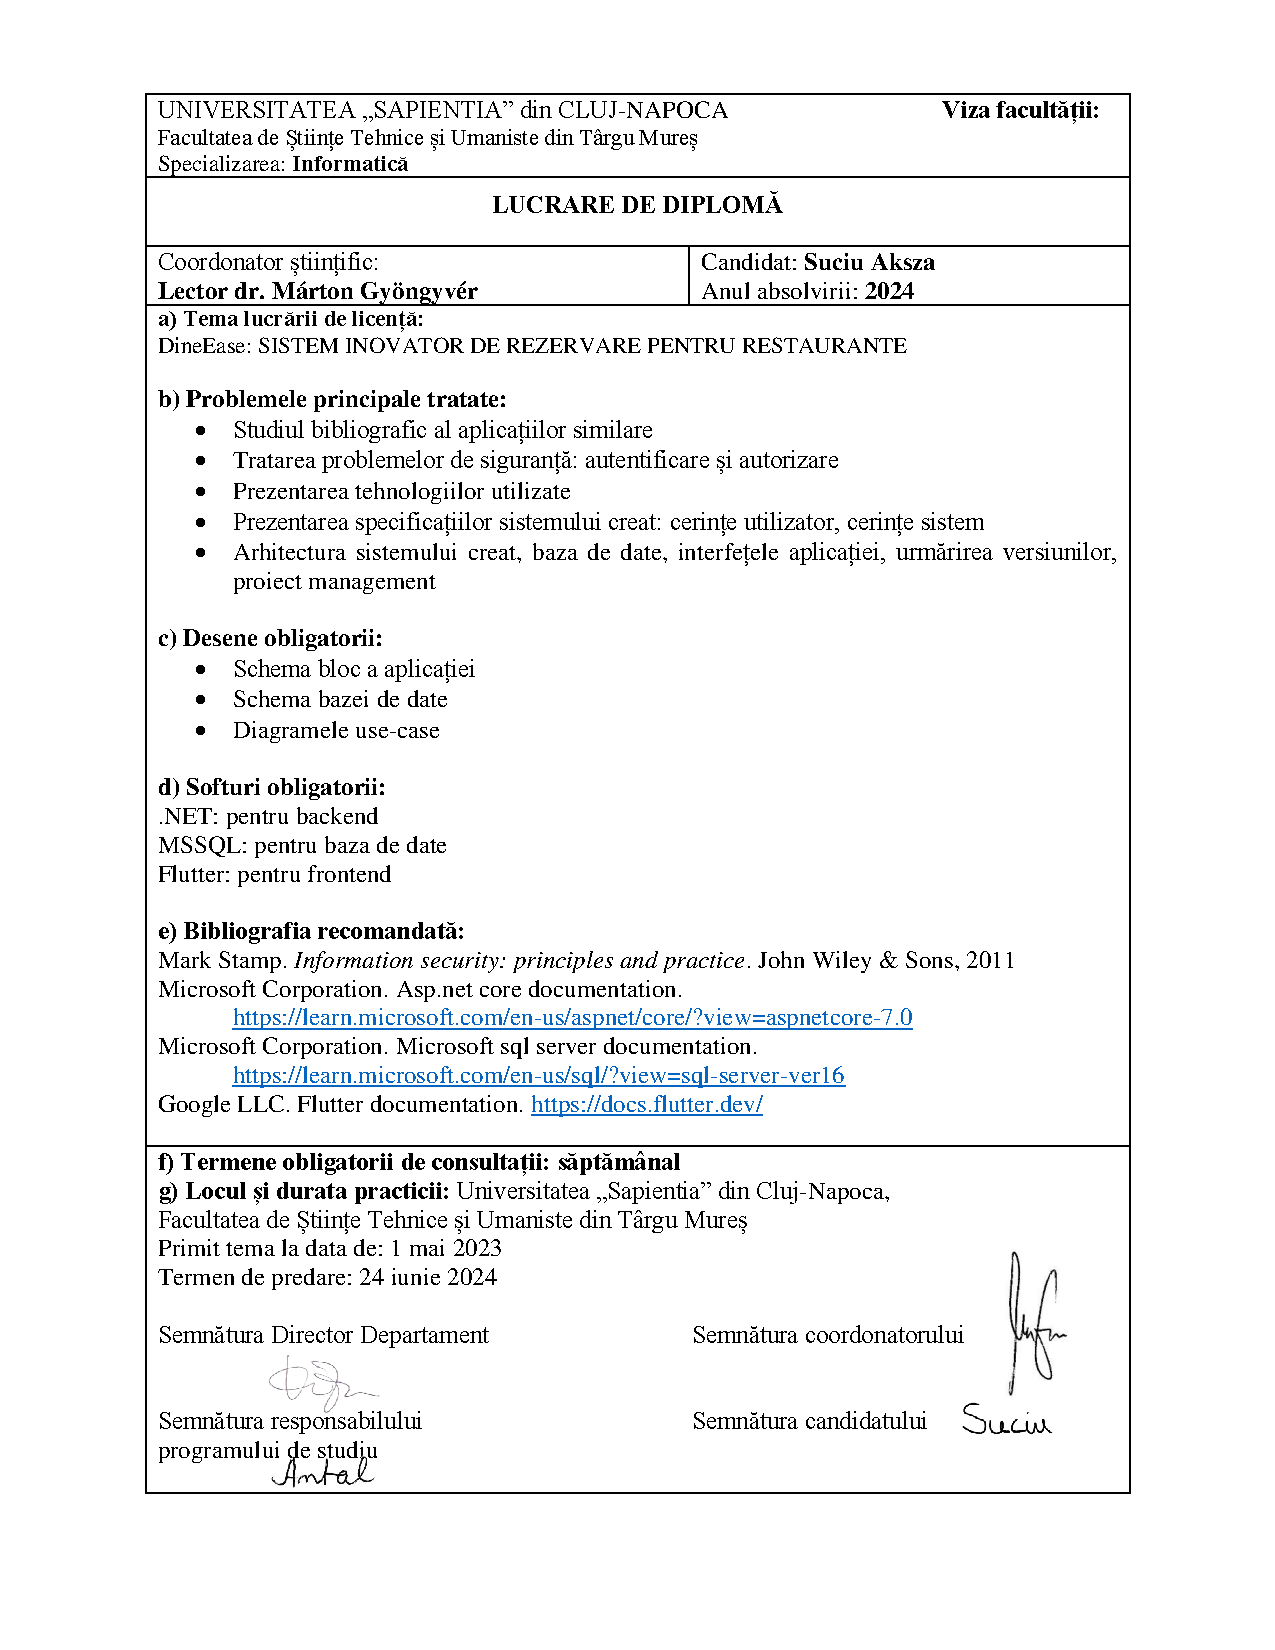
\includepdf[pages={1}]{content/SuciuAksza.pdf}
	
\includepdf[pages={1}]{content/Declaratie.pdf}
	\pagenumbering{gobble}

\selectlanguage{magyar}
\hungarianParagraph

%----------------------------------------------------------------------------
% Abstract in Hungarian
%----------------------------------------------------------------------------

\chapter*{Kivonat}

A dolgozatom egy mesterséges intelligenciával támogatott beszédfejlesztő alkalmazás tervezését és megvalósítását mutatja be. A hagyományos nyelvtanulási módszerek gyakran a nyelvtani szabályok és az elszigetelt szókincs elsajátítására helyezik a hangsúlyt, miközben korlátozott lehetőséget biztosítanak a valós kommunikáció gyakorlására. Ennek következtében a tanulók nehezebben alkalmazzák tudásukat valódi beszédhelyzetben.

A fejlesztett alkalmazás célja, hogy beszélgetésalapú tanulási környezetet biztosítson, ahol a felhasználók mesterséges intelligenciával folytatott párbeszédek során fejleszthetik nyelvi készségeiket. Az AI automatikusan felismeri, kijavítja a hibáikat, majd segít nekik a fejlődésben azzal hogy ismételten előkerülnek ezek a beszélgetések során.

A dolgozat bemutatja az alkalmazás felépítését, a megvalósítás során alkalmazott módszereket és technológiai megoldásokat, valamint azt, hogy a beszélgetésközpontú, hibaalapú tanulási megközelítés miként járult hozzá a beszédkészség hatékony fejlesztéséhez.

\vfill
\selectlanguage{romanian}

%----------------------------------------------------------------------------
% Abstract in Romanian
%----------------------------------------------------------------------------
\chapter*{Rezumat}

Lucrarea mea prezintă proiectarea și implementarea unei aplicații de dezvoltare a abilităților de vorbire, susținută de inteligență artificială. Metodele tradiționale de învățare a limbilor străine pun adesea accentul pe însușirea regulilor gramaticale și a vocabularului izolat, oferind în același timp oportunități limitate pentru exersarea comunicării reale. Ca urmare, cursanții întâmpină dificultăți în aplicarea cunoștințelor dobândite în situații reale de vorbire.

Scopul aplicației dezvoltate este de a oferi un mediu de învățare bazat pe conversație, în care utilizatorii își pot dezvolta competențele lingvistice prin dialoguri purtate cu o inteligență artificială. AI-ul identifică și corectează automat greșelile utilizatorilor și sprijină procesul de învățare prin reluarea acestora în cadrul conversațiilor ulterioare.

Lucrarea prezintă structura aplicației, metodele și soluțiile tehnologice utilizate în procesul de implementare, precum și modul în care abordarea de învățare centrată pe conversație și pe greșeli contribuie la dezvoltarea eficientă a abilităților de comunicare orală.

\vfill
\selectlanguage{english}
%\englishParagraph

%----------------------------------------------------------------------------
% Abstract in English
%----------------------------------------------------------------------------
\chapter*{Abstract}

This thesis presents the design and implementation of an artificial intelligence–supported application for the development of speaking skills. Traditional language learning methods often emphasize the acquisition of grammatical rules and isolated vocabulary, while providing limited opportunities for practicing real-life communication. As a result, learners face difficulties in applying their knowledge in authentic speaking situations.

The aim of the developed application is to provide a conversation-based learning environment in which users can improve their language skills through dialogues with an artificial intelligence. The AI automatically identifies and corrects users’ errors and supports their progress by revisiting these mistakes during subsequent conversations.

The thesis describes the structure of the application, the methods and technological solutions applied during its implementation, and examines how a conversation-centered, error-based learning approach contributes to the effective development of speaking skills.


\vfill
\dolgozatnyelve
\defaultParagraph
 
% Tartalomjegyzek
%~~~~~~~~~~~~~~~~~~~~~~~~~~~~~~~~~~~~~~~~~~~~~~~~~~~~~~~~~~~~~~~~~~~~~~~~~~~~~~~~~~~~~~
	\pagenumbering{arabic}
	\setcounter{page}{9}
	\tableofcontents\vfill

% A diplomadolgozat lenyegi resze
%~~~~~~~~~~~~~~~~~~~~~~~~~~~~~~~~~~~~~~~~~~~~~~~~~~~~~~~~~~~~~~~~~~~~~~~~~~~~~~~~~~~~~~


	%----------------------------------------------------------------------------
\chapter{Bevezető}%\addcontentsline{toc}{chapter}{Bevezető}
%----------------------------------------------------------------------------

Sok nyelvtanuló szembesül azzal a problémával, hogy bár hosszú időn keresztül tanul egy idegen nyelvet, mégsem érzi magát magabiztosnak, amikor valódi beszédhelyzetbe kerül. Gyakran előfordul, hogy az elsajátított tudása ellenére nehézséget jelent egy egyszerű párbeszéd lebonyolítása is, vagy a gondolatok megfogalmazása. Sokszor hallhatjuk azt is, hogy egy nyelvet akkor lehet igazán megtanulni, ha azt aktívan használjuk\cite{swain1985communicative,long1996role}, azonban erre nem minden tanulónak van lehetősége. Különösen igaz ez azokra, akiknek a környezetükben nincs olyan személy, akivel rendszeresen gyakorolhatnák a nyelvet.

A hagyományos nyelvtanulási módszerek és alkalmazások jellemzően nyelvtani szabályokra, elszigetelt szókincs elsajátítására helyezik a hangsúlyt. Bár ezek fontos elemei a nyelvtanulásnak, gyakran kevés figyelem jut a beszédkészség fejlesztésére és a valós kommunikáció gyakorlására. \cite{swain1985communicative,long1996role}

Ezekre a problémákra szeretnék megoldást nyújtani az általam fejlesztett alkalmazással, amely egy mesterséges intelligenciával támogatott beszédalapú nyelvtanulási környezetet biztosít. Az alkalmazás lehetőséget nyújt arra, hogy a felhasználók mesterséges intelligenciával folytatott párbeszédek során gyakorolhatják a célnyelvet, mintha egy valódi beszélgetőpartnerrel kommunikálnának. \cite{xiao2024conversational} Az AI nemcsak részt vesz a beszélgetésben, hanem felismeri és kijavítja a nyelvi hibákat \cite{lyster2013oral,sato2012peer}, illetve eltárolja azokat, későbbi feldolgozás céljából.

A rendszerben külön figyelem irányul arra, hogy a felhasználók ne csupán javítást kapjanak, hanem lehetőséget arra is, hogy saját hibáikból tanuljanak. A gyakran előforduló hibák ismételten megjelennek a tanulási folyamat, beszélgetések és különböző gyakorlási módszerek segítségével, így elősegítve a helyes nyelvi minták rögzülését és a beszédkészség folyamatos fejlődését.

A következő fejezetekben bemutatom az alkalmazás tervezésének és megvalósításának folyamatát, az alkalmazott módszereket és technológiai megoldásokat, valamint elemzem, hogy a beszélgetésközpontú, hibaalapú megközelítés miként járul hozzá a hatékony nyelvtanuláshoz és a beszédkészség fejlesztéséhez.

	%----------------------------------------------------------------------------
\chapter{Hasonló alkalmazások, felhasznált technológiák} \label{fejezet3}
%----------------------------------------------------------------------------

\section {Hasonló alkalmazások}

Dolgozatom ezen részében először megvizsgálunk néhány olyan alkalmazást, amelyek hasonló feladatot végeznek, mint az általam megvalósított alkalmazásunk.

A piacon található néhány nyelvtanuló alkalmazás, amelyek hasonló funkcionalitásokkal vannak ellátva, mint az Echo alkalmazás. Dolgozatom során megvizsgáltam több alkalmazást is, és elmondható róluk hogy felépítésük hasonló, ugyanakkor az Echo alkalmazás egyedisége e beszéd fókuszú tanulásban rejlik.

A vizsgált alkalmazások között szerepelnek a következők: 

\href{https://play.google.com/store/apps/details?id=com.selabs.speak}{Speak: Language Learning} \cite{speak}, \href{https://play.google.com/store/apps/details?id=ai.praktika.android&hl=en}{Praktika: AI learning tutor} \cite{praktika}, \href{https://play.google.com/store/apps/details?id=com.duolingo&hl=en}{Duolingo}\cite{duolingoMax}.

Ezek az alkalmazások mind nyelvoktatással foglalkoznak, különböző megközelítésben. A Speak és a Praktika leginkább beszédfejlesztésre fókuszál, különböző szituációs beszélgetéseket ad a felhasználónak, amellyel támogatja a kommunikációs készségét az idegen nyelven. A Duolingonak is van egy hasonló funkciója, amelyben kommunikációt lehet fejleszteni, viszont ez az alkalmazás inkább szókics bővítésre, nyelvtani szabályok elsajátítására használatos.

A Speak alkalmazás AIal való beszélgetést támogat, különböző témakörökben. Ez képes elemezni a beszédet, visszajelzést ad a kiejtésről, javaslatokat ad mondatszerkesztésre. \cite{speakAppStore} Ez az alkalmazás a leghasonlóbb az általunk fejlesztett alkalmazáshoz.

A Praktika ugyanúgy a mesterséges intelligencia segítségét hívja segítségül a nyelvtanulásban, viszont ebben az alkalmazásban különböző avatarokkal beszélgethetük, így még személyesebbé és még reálisabbá téve a kommunikációt a felhasználó számára.\cite{praktikaGooglePlay}

A Duolingo a legelterjedtebb alkalmazás, amely elsősorban szókincs bővítésére hasznos.\cite{duolingoMax} Játékos felülete vonzóvá teszi a felhasználónak az alkalmazás használát. A beszélgető mód a fizetős verzióban érvényes, itt is mesterséges intelligencia használatával, viszont a hangsúlya az alkalmazásnak nem feltétlenül ezen van.

A vizsgált alkalmazások közös jellemzője természetesen az, hogy mindegyik a nyelvtanulást támogatja és van nekik AIal támogatott verizójuk is. Legtöbbüknél ez a funkció fizetős. Ezekben az alkalmazásokban ugyanúgy lehet profilt készíteni, támogatják azt, hogy nap mint nap gyakorolja a felhasználó az adott nyelvet, illetve statisztikákat is megtekinthetnek a fejlődésükről.

Ezekben az alkalmazásokban fellelhető a jól ismert gamifikáció is. Ennek célja az, hogy a felhasználó játszva tanuljon, jól érezze magát, jutalmazva érezze magát tanulás közben. \cite{deterding2011gamification} Ezzel a módszerrel könnyebben meggyőzhetik a fejlesztők a felhasználókat, hogy szívesebben használják az alkalmazást, ezzel motiválva őket a fejlődésre.

Összességében elmondható hogy ezek az alkalmazások különböző igényekhez mérten, hatékony megoldásokat kínálnak a nyelvtanulásra. A legtöbb alkalmazás vagy gamifikációra vagy előre meghatározott feladatokkal segíti a tanulást. A megvalósított alkalmazás célja ezzel szemben az, hogy a felhasználók számára egy olyan platformot biztosítson, ahol a hangsúly elsősorban a valós idejű beszélgetésen és kommunikációs készsegek fejlesztéseén van mesterséges intelligencia segítségével.

\section{Felhasznált technológiák}

Az előzőleg felsorolt alkalmazások nagyrészt hasonló technológiákat használnak. Mobil frontendnek a React Native nyelvet használják, cloud infrastructure, illetve NLP modelleket használnak valósidejű hangfeldolgozás és generálás céljából. Egyetlen eltérés a Duolingo alkalmazásnál van. Lévén, hogy egy régebbi alkalmazásról beszélünk, inkább az akkori trendeket követve másfajta technológiákat használt, ellenben az előzőleg felsorolt alkalmazásokkal, amelyek nem olyan rég készültek. A Duolingo Kotlint használ modern Android fejlesztés céljából, a backend technológiája pedig a népszerű Python nyelven íródott, amely könnyen használható machine learninghez. AI szempontjából vizsgálva GPT 4 integrációt használtak fel az alkalmazásban, amivel biztosítják az interaktívabb feladatokat és valósidejű beszélgetésekhez használják.

A következő alfejezetekben röviden bemutatom az általam felhasznált technológiákat.

\subsection{Flutter}

A Flutter Google által fejlesztett nyílt forráskódú keretrendszer, amelyet UI fejlesztésére használnak. Ez lehetővé teszi a keresztplatformos alkalmazások fejlesztését egyetlen kódbázisból. A projekt frontendje ebben a keretrendszerben valósult meg, mivel modern felhasználói felületet biztosít különböző csomagok segítségével, illetve jól integrálható backend szolgáltatással. \cite{flutter}


\subsection{ASP.NET Core}

Az ASP.NET Core nyílt forráskódú webes keretrendszer, amelyet a Microsoft hozott létre. A keretrendszer segítségével komplex alkalmazások backendjét hozhatjuk létre, amelyek gyorsak és skálázhatók. Ez olyan API tervezéséhez és elkészítéséhez járul hozzá, amely segít hatékonyan adatáramlást elérni az adatbázis vagy az AI modell és a kliensalkalmazás között. \cite{aspnetcore}

\subsection{Microsoft SQL Server}

A Microsoft SQL Server (MSSQL) relációs adatbáziskezelő rendszer, amely nagy mennyiségű adatok tárolását és kezelését teszi lehetővé. Ez az adatbáziskezelő nagyon egyszerűen integrálható a .NET keretrendszerrel, lévén hogy Microsoft által fejlesztették őket.\cite{mssql}

\subsection{Python}
A Python magasszintű programozási nyelv, amely széles körben elterjedt, leginkább mesterséges intelligencia és gépi tanulás területén. Az alkalmazás AI funkciói külön Python alapú mikroszolgáltatásokként kerültek megvalósításra. \cite{python}

A felhasznált AI-ok a következőkben lesznek bemutatva

\subsubsection{Faster-Whisper}
A Whisper beszédfelismerő modell optimizált változata ez. Ez hozzájárul az alkalmazásban a felhasználó hangüzeneteinek szöveggé alakítására, amikor konverszációt kezdeményez a felhasználó, az ő beszédét alakítja át írásos formába.\cite{fasterwhisper,whisper}

\subsubsection{Phi3-Mini}
A Phi3 egy kisméretű nyelvi modell, amely természetes nyelvű válaszok generálására és szövegfeldolgozásra alkalmas. A rendszerben ez végzi a beszélgetések kezelését, valamint nyelvi hibák felismerését és javítását. \cite{phi3}

\subsubsection{Piper TTS}
A Piper egy nyílt forráskódú text to speech rendszer, amely képes a szöveget beszéddé alakítani. Az alkalmazásban az AI által generált válaszok hangos felolvasására szolgál. \cite{piper}
	%----------------------------------------------------------------------------
\chapter{Rendszer specifikációja}
%----------------------------------------------------------------------------

\section {Felhasználói követelmények}

Egyetlen felhasználói típusunk van az applikációban: a tanuló, amely nyelvi készségeit fejleszteni kívánja.

\begin{itemize}
    \item \textbf{Platform}
    
    Egy mobilalkalmazás formájában a tanulni vágyó felhasználók mesterséges intelligencia segítségével gyakorolhatják a célnyelvet, ahol fejlődésüket tudják követni, különböző gyakorló feladatokat végezni és a beszédkészségükön dolgozni.

    \item \textbf{Regisztráció oldal}

    A felhasználó a szükséges adatok megadásával fiókot hozhat létre a platformon. Ennek elvégzése után kaphat hozzáférést az alkalmazás lényegi funkcióihoz.

    \item \textbf{Bejelentkezés oldal}

    A már létrehozott fiókba bejelentkezhet a felhasználó az email cím és jelszó megadásával. Sikeres bejelentkezés után pedig máris nekiláthat a nyelvtanulásnak.

    \item \textbf{Onboarding oldal}

    Az első bejelentkezés után a felhasználó kiválaszthatja a tanulni kívánt nyelvet, tanulási célját és egy kis felmérés után személyre szabott rendszert használhatja.

    \item \textbf{Főoldal}

    A főoldalon a felhasználó több gombbal is találkozik, amelyek különböző oldalakra vezetnek. Itt megtekintheti a legutóbbi beszélgetéseket, napi ajánlásokat, hiba összegzéseket, illetve egy gomb segítségével azonnal beszélgetést indíthat a mesterséges intelligenciával. Ugyanitt láthatja a profil oldalát is illetve a gyakorlást indító gombot is. Az oldal célja, hogy egy egységes helyen megtalálhassa a fő funkciókat a felhasználó.

    \item \textbf{Napi ajánlás oldal}

    Személyre szabott ajánlásokkal találkozhatnak ezen az oldalon a felhasználók. Ez tartalmaz gyakorló feladatokat, ismétlődő hibákat, ajánlott beszélgetési témákat.

\newpage
    \item \textbf{Előzmények}

    Ezen az oldalon visszakövetheti a felhasználó korábbi beszélgetési témáit, hibáit ezekben a beszélgetésekben, összefoglalókat róla. Ez segít az ismétlésben, és a fejlődés megfigyelésében is.

    \item \textbf{Hibák összegzése, Szótár}

    Ez az oldal arra szolgál, hogy a felhasználó megtekintse korábbi hibáit, javításokat, magyarázatokat. Segíti a tudatos tanulást az, hogy repetitíven  tanulhat a felhasználó.

    \item \textbf{Beszélgetés oldal}

    A platform a beszédfejlesztésre fókuszál leginkább, így elsősorban beszédben kommunikálhat a mesterséges intelligenciával különböző témákban. Ez feldolgozza a beszédet, válaszol, javítja a hibákat. Opcionálisan találunk itt egy chat felületet, ahol esetlegesen az AI által meg nem értett szavakat vagy mondatokat gépelhet a felhasználó és erre kap választ. Azt fontos kiemelni, hogy ezen az oldalon elérhető egy gomb, amellyel feliratozhatja a mesterséges intelligencia válaszait, vagy akár a sajátjait is.

    \item \textbf{Gyakorlás oldal}

    Több fajta gyakorlásból választhat a felhasználó, amely segíti úgy a beszédkészségét mint az írás- olvasás készségeit is. Flashcard vagy Pronunciation card funkcióval a felhasználó megtanulhatja különböző szavak kiejtését és jelentését is. Correct the sentence vagy Fill in the gap funkcióval gyakorolhatja a helyes beszédet, ezen az oldalon felhasználva vannak a tanuló hibái is, ahhoz hasonló mondatokat kell kijavítania. 

    \item \textbf{Profil}

    A felhasználó ezen az oldalon megtekintheti adatait, fejlődését, változtathat különböző személyes információin.

    \item \textbf{Statisztikák}

    Grafikus formában is elérhetőek a tanulók fejlődési adatai, hibái, aktivitása.

    \item \textbf{Beállítások, Mesterséges intelligencia személyre szabása}

    Ezen az oldalon lehetősége nyílik a felhasználónak módosítani tanulásán. Változtathat itt nyelvi, illetve AI beállításokat.
    
\end{itemize}

A következő \ref{fig:usecase} ábrán bemutatom egy diagram segítségével a felhasználói use case-eket, amelyek az alkalmazásban elérhetőek.

\begin{figure}[ht]
    \centering
    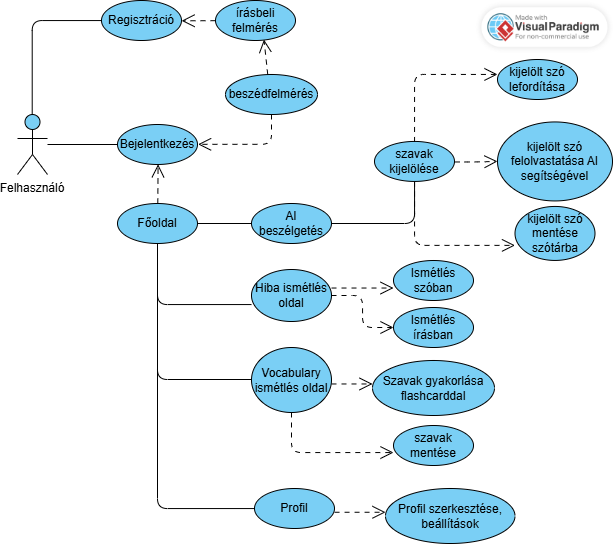
\includegraphics[width=0.9\linewidth]{images/image.png}
    \caption{Felhasználói use case diagram}
    \label{fig:usecase}
\end{figure}



\newpage

\section {Rendszerkövetelmények}

\subsection{Funkcionális követelmények}

Az alábbiakban bemutatok minden fontos funkciót az alkalmazásból.

\begin{itemize}
    \item \textbf{Regisztráció}

    A rendszer lehetőséget biztosít a felhasználó számára egy új fiók létrehozására. A regisztráció során a felhasználónak meg kell adnia a szükséges adatait. A rendszer ellenőrzni az adatokat, és hogy ki van-e töltve minden mező, formátumot ellenőriz. Ezek után ha hibát észlel a rendszer, akkor hibaüzenetet jelenít meg. A sikeres regisztráció esetén a felhasználó adatai biztonságosan eltárolásra kerülnek az adatbázisban, titkosított formában.\cite{owaspPasswordStorage}

    \item \textbf{Bejelentkezés}

    Ha már létrehozott egy fiókot a felhasználó, akkor lehetősége nyílik bejelentkezni a meglévő fiókjába. A felhasználónak meg kell adnia email címét és jelszavát. Nem megfelelő adatok esetén visszajelzést küld a hibáról a rendszer, sikeres bejelentkezés esetén pedig a rendszer hitelesítési tokent generál \cite{jwt}, amely lehetővé teszi a felhasználó számára az alkalmazás további, főbb funkcióit.

    \item \textbf{Beszélgetés a mesterséges intelligenciával}

    Az applikáción belül a felhasználóknak van lehetőségük a mesterséges intelligenciával folytatott beszélgetésre, a célnyelven. A felhasználó hang alapúan beszélgethet, vagy akár néhány mondatot írásban is küldhet a mesterséges intelligenciának. A rendszer célja, hogy a beszélgetés minél inkább hasonlítson egy valós kommunikációs helyzethez. Ennek segítségével a felhasználó tanulhatja a magabiztosabb kommunikációt.

    \item \textbf{Hibák felismerése és kezelése}

    A beszélgetés során a rendszer automatikusan felismeri a felhasználó által elkövetett nyelvi hibákat. Ezeket a hibákat kijavítja, majd eltárolja az adatbázisban, kiegészítve a helyes megoldással és szükség esetén magyarázattal. A hibák később visszakereshetők és felhasználhatók a tanulási folyamat támogatására.

    \item \textbf{Gyakorló feladatok generálása}

    A rendszer képes a felhasználó korábbi hibái alapján személyre szabott gyakorló feladatok generálására. Ezek a feladatok különböző típusúak lehetnek, például hiányos mondatok, kiejtés tanulás, szókincs alapú feladatok. A cél, hogy a felhasználó ismételten találkozzon a hibáival, és ezáltal hatékonyabban rögzítse a helyes nyelvi formákat.

    \item \textbf{Előzmények kezelése}

    A rendszer nem tárolja el a felhasználók korábbi beszélgetéseit, biztonsági okokból, viszont eltárolja a beszélgetések témájának címét, összefoglalót róla, és a hibákat, megjegyzéseket. Ennek segítségével a felhasználó nyomon tudja követni fejlődését és visszatérhet korábbi tanulási helyzetekhez.

    \item \textbf{Statisztikák}

    A rendszer különböző statisztikai adatokat gyűjt és jelenít meg a felhasználó számára, mint például a beszélgetések száma, hibák mennyisége, fejlődés üteme. Ezek az adatok segítik a felhasználót abban, hogy jobban átlássa a tanulási folyamatát.

    \item \textbf{Profil}

    A felhasználó megtekintheti és módosíthatja saját adatait a profil oldalon. Itt lehetősége nyílik a személyes beállítások, például a nyelvi szint vagy a tanulási célok módosítására.

    \item \textbf{Mesterséges intelligencia beállítások kezelése}

    A rendszer lehetőséget biztosít különböző beállítások módosítására, mint például az alkalmazás nyelve, az értesítések kezelése, az AI viselkedésének testreszabása. Ezek a beállítások hozzájárulnak a felhasználói élmény személyre szabásához.

\end{itemize}

\newpage


\newpage
\subsection{Nem funkcionális követelmények}

 Az applikáció mobil alkalmazásnak lett elkészítve, ugyanakkor a Flutter \cite{flutter} keretrendszernek köszönhetően más platformokon is használható. Gyors és stabil nyelvtanulási környezet biztosítása a cél, amely támogatja a mesterséges intelligenciával történő kommunikációt és beszédfejlesztést.

\begin{itemize}
    \item \textbf{Operációs rendszer}
    
    Az alkalmazás Android operációs rendszerre lett elkészítve, viszont más platformokon is működik. A legmegfelelőbb verziók vagy böngészők a különböző platformokon a következőek:
     \begin{itemize}
        \item \textit{Android:} 5.0 vagy újabb
        \item \textit{Web:} Google Chrome, Mozilla Firefox, Microsoft Edge aktuális verziói
     \end{itemize}
    Az alkalmazás fejlesztése során fontos szempont volt, hogy különböző képernyőméreteken és eszközökön is megfelelő felhasználói élményt nyújtson.

    \item \textbf{Tárhely}
    Az alkalmazás telepítéséhez és működéséhez legalább 250MB szabad tárhely szükséges. Később ez nőhet, eltárolt hangfájlok vagy gyorsítótározott adatok mennyiségétől függően.

    \item \textbf{Internetkapcsolat}

    Aktív internetkapcsolatra van szükség az alkalmazás működéséhez, mivel a mesterséges intelligenciával történő kommunikáció, a beszédfelismerés, valamint az adatok szinkronizálása szerveroldalon történik. Internetkapcsolat hiányában az alkalmazás bizonyos funkciói nem lesznek elérhetőek.

    \item \textbf{Teljesítmény}

    Egy nagyon fontos követelmény a gyors válaszidő. Különösen fontos szempont ez a beszélgetések során, ahol a felhasználó valós idejű kommunikációs élményt vár el. Az AI válaszgenerálásának, a beszédfeldolgozásnak és az adatbázislekérdezéseknek optimalizált módon kell működnie, azért hogy az alkalmazás folyamatos és gördülékeny felhasználói élményt biztosítson.

    \item \textbf{Megbízhatóság}

    A fejlesztés során fontos szempont volt a stabil működés és a hibák megfelelő kezelése. Különböző hibakezelési mechanizmusokat alkalmazunk annak érdekében, hogy egy esetleges hiba ne okozza az alkalmazás leállását. A backend oldalon központi hibakezelés került kialakításra, amely lehetőséget nyújt megfelelő válaszok visszaküldését a kliens számára.

    \item \textbf{Skálázhatóság}
    A rendszer úgy lett kialakítva, hogy lehetővé tehesse a további funkciók és szolgáltatások későbbi integrálását. Az AI szolgáltatások külön microszervizekként lettek elkészítve, így a rendszer könnyen bővíthetővé és fejleszthetővé vált. \cite{fowlerMicroservices} Ez lehetőség az új modellek, nyelvek, tanulási funkciók hozzáadására, anélkül hogy a teljes rendszer architektúráján módosítani kellene.

    \item \textbf{Modularitás}
    Az alkalmazás, köszönhetően a funkciók egymástól elkülönítésének, moduláris felépítést alkalmaz. Ez megkönnyíti a komponensek fejlesztését, tesztelését, cseréjét. A frontend, backend, AI szolgáltatások mind különálló részekként működnek a rendszerben.

    \item \textbf{Bővíthetőség}
    A rendszer tervezésénél a jövőre is gondoltam. Úgy lett megtervezve, hogy később új gyakorlási módokkal, új AI funkciókkal vagy további nyelvekkel bővíthető legyen. Ez a megközelítés lehetővé teszi az új módulok hozzáadását, anélkül hogy jelentős változásokat kellene végrehajtani a rendszerben.
    
\end{itemize}

	%----------------------------------------------------------------------------
\chapter{Tervezés}
%----------------------------------------------------------------------------

\section{Szoftver terv}

A rendszer architektúrája a következő komponensekből tevődik össze: felhasználói interfész, backend API, mesterséges intelligencia szolgáltatásai, adatbázis. Ez a több komponenses felépítés működtetéséhez szükséges az internetkapcsolat, amely a kommunikációhoz segít hozzá a komponensek között. A rendszer architektúráját a következő ábra szemlélteti, ahol megfigyelhető a részek közötti kapcsolat és adatáramlás.

\begin{figure}[ht]
    \centering
    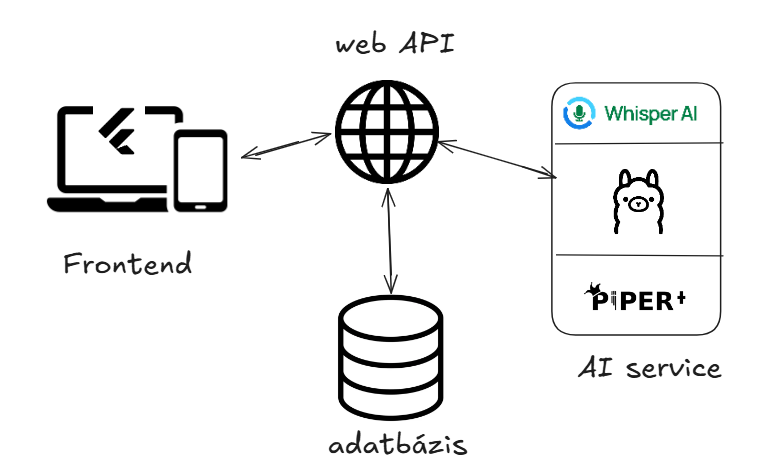
\includegraphics[width=0.8\linewidth]{images/rendszer.png}
    \caption{Rendszer architektúrája}
    \label{fig:arch}
\end{figure}
\newpage

\subsection{Logikai nézet}

A felhasználói felület egy Flutter framework segítségével fejlesztett mobilalkalmazás. Ez lehetővé teszi a cross platform alkalmazások készítését, így az alkalmazásunk amelyet eredetileg mobilra fejlesztettem, könnyedén futtatható weben, akár desktopon is. A felhasználók ezen a területen érhetik el az alkalmazás funkcióit, mint a beszélgetéseket, gyakorló feladatokat, fejlődésükről való statisztikákat.

A backend rétegért a .NET alapú Web API felelős, amely üzleti logikát, autentikációt, adatkezelést, frontend és adatbázis közötti kommunikációt is végrehajt. Az API fogadja a kliens kéréseit, feldolgozza azokat, majd visszaküldi a megfelelő válaszokat.

A rendszer lelke, legfontosabb része: az API szervíz, amely Python alapú réteg. Itt valósulnak meg a mesterséges intelligenciával kapcsolatos funkciók. Ez a komponens felelős többek között a beszédfelismerésért, a nyelvi hibák felismeréséért és javításáért, válasz generálásért, nem utolsó sorban pedig a szöveg felolvasásáért. Az AI szolgáltatások külön komponensekként működnek, amelyekkel a backend API kommunikál. \cite{fowlerMicroservices} Az AI szolgáltatások, amelyek a beszélgetéshez hozzájárulnak azok a Whisper, Phi3, Piper szolgáltatás. A konkrét flow, ami végigmegy ezeken az AI-okon: amikor a felhasználó beszél a mesterséges intelligenciához, akkor a Whisper dolgozza fel a beszédet, amelyet átalakít szöveggé, ezt a szöveget átadja a Phi3 LLM modellnek \cite{whisper,fasterwhisper,phi3,piper}, amely többek között a választ generálja a szövegre, így szimulálva a valós beszélgetést, ezt a választ viszont szövegként adja vissza a Phi3 modellünk, így végezetül a Piper AI modell alakítja át a szöveget hanggá, biztosítva a valós beszélgetés érzetét.

Az adatok tárolásához egy MSSQL adatbázist használunk. Itt kerülnek eltárolásra a felhasználói adatok, beszélgetés címek, hibák, gyakorlási adatok és statisztikák. Az adatbázis kezeléséhez Code First megközelítést alkalmaztam Entity Framework segítségével, amely lehetővé teszi az adatmodellek egyszerű kezelését és migrációk használatát. \cite{efcoreMigrations}

A komponensek közötti kommunikáció internetkapcsolat segítségével megvalósított. A felhasználói felületről érkező kérések először a backend APIhoz kerülnek, amely szükség esetén kommunikál az AI szolgáltatásokkal vagy az adatbázissal. A feldolgozott válasz ezután visszakerül a kliens alkalmazásba.


\subsection{Folyamat nézet}

Az alábbiakban néhány lényeges folyamatot mutatok be, hogy hogyan viselkednek különböző részei a rendszernek.

\begin{enumerate}
    \item \textbf{Hangalapú beszélgetés}
    \begin{itemize}
        \item A felhasználó hangüzenetet küld az alkalmazás számára
        \item A hangfájlt elküldjük az APIn keresztül az AI szolgáltatáshoz
        \item A továbbítás után speech to text AI modell szöveggé alakítja a beszédet
        \item Az AI feldolgozza a szöveges üzenetet, ehhez választ generál és megállapítja a hibákat, amelyeket json formátumban küld vissza az endpointban
        \item A generált választ text to speech AI áltat hanggá alakítjuk, ezt eltároljuk egy mappába
        \item Az elkészült válasz visszakerül a felhasználói felületre és a hang megszólal, de újrajátszható is lesz a hang egy gomb segítségével, és a szavakat is fel lehet mondatni az AI segítségével egy kattintással.
    \end{itemize}
    \item \textbf{Hibák felismerése és eltárolása}
    \begin{itemize}
        \item Amikor a felhasználó az AI modellel beszélget, akkor az AI elemzi a felhasználó válaszai helyességét.
        \item Ha nyelvi hibát észlel automatikusan eltárolja azt a hibák közé, csoportosítja azt, és magyarázatot is generál
        \item Ez majd a gyakorláson alapuló tanuláshoz járul hozzá.
    \end{itemize}
    \item \textbf{Gyakorló feladat generálása}
    \begin{itemize}
        \item A rendszer lekéri a felhasználó hibáit az adatbázisból
        \item A felhasználó tud írásban vagy hangban is gyakorolni, hangban azért nehezebb de hatékonyabb, mert az AI érzékeny az akcentusra és a hanglejtésre is
        \item Gyakorlatilag a felhasználónak ki kell javítani az előzőekben elkövetett hibáit
        \item A felhasználó válaszát az AI javítja ki
        \item Ezen gyakorlatok eredményei eltárolódnak az adatbázisban
        \item Ezek a gyakorlatok hozzájárulnak a felhasználó fejlődéséhez, az eltárolt adatai pedig a statisztikákhoz és mérésekhez
    \end{itemize}
    \item \textbf{Statisztikák frissítése}
    \begin{itemize}
        \item A rendszer a beszélgetések és gyakorlások során különböző adatokat gyűjt a felhasználó aktivitásáról
        \item Ezeket az adatokat az adatbázisban tároljuk el
        \item Az API feldolgozza az adatokat és statisztikákat készít, mint például a hibák száma, gyakorlások száma, fejlődési tendencia
        \item A statisztikák megjelennek a felhasználó profilján és statisztikai felületén
    \end{itemize}
\end{enumerate}

\newpage
\section{Adatbázis terv}

\begin{figure}[ht]
    \centering
    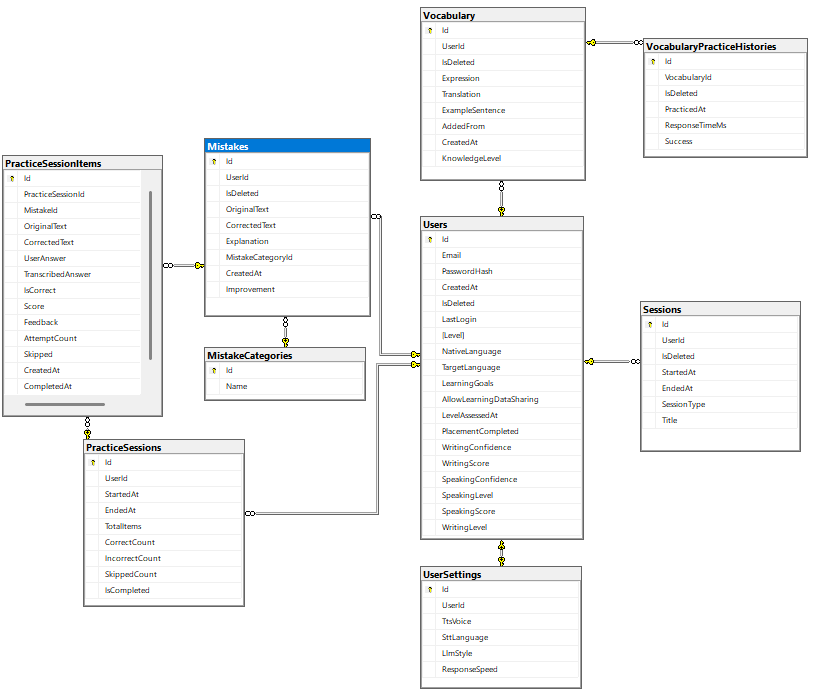
\includegraphics[width=0.8\linewidth]{images/adatbazis2.png}
    \caption{Adatbázis terv}
    \label{fig:database}
\end{figure}
Az adatbázist relációs adatbázisként terveztem meg, amely mindössze 9 táblával rendelkezik. Ezekben a táblákban tárolom el a felhasználó adatait, gyakorlatait. Ezek hozzájárulnak az aplikáció megfelelő működéséhez.

Ezekben a táblákban a legnagyobb a felhasználó adatait tartalmazó tábla, ez egy nagyon fontos hely, amiben sok lényeges adat van eltárolva, ezek mind hozzásegítenek a fejlődés méréséhez és magához a fejlődéshez is, mivel az AI ehhez mérten válaszol neki.

A Vocabulary  táblában mentődik el minden olyan szó vagy szókapcsolat, amelyet a felhasználó nem ismert és ezeknek fordítása. Ezeket a szavakat elmentheti a felhasználó manuálisan, ha bárhol is szembejön vele és szeretne egy olyan helyre menteni, ahol majd előveheti és gyakorolhatja azt, illetve a mesterséges intelligenciával történő beszélgetés során is hozzáadhat ehhez a táblához.
A VocabularyPracticeHistory tábla a Vocabulary-ba eltárolt kifejezések tanulásához járul hozzá. Mivel flashcardok segítségével gyakorolhatja ezeket a felhasználó, itt tárolódik el a helyessége, a válaszidője, és minden más fontos adat, amelyet felhasználhatunk a fejlődés elemzésére.

A Mistakes tábla az azok a szókapcsolatok vagy mondatok tárhelye és azoknak javított verziója, amelyeket a felhasználó elhibázott beszélgetés közben. Mindez úgy tárolódik el ebbe a táblába, hogy beszélgetés közben a mesterséges intelligencia figyeli, milyen hibákat vét a felhasználó és mindezt elmenti kijavított verziójával együtt és magyarázattal. 
Ezeket a hibákat nem hiába mentjük el, ugyanis gyakorló feladatokkal megtanítjuk a helyes verzióját ezeknek. A PracticeSessions és PracticeSessionItems ezért is kapcsolódik a Mistake táblához, mivel a felhasználó gyakorlását ide tároljuk el, minden egyes adatot róla.

A Sessions tábla a mesterséges intelligenciával való beszélgetésről tárol összefoglaló címet, mivelhogy a felhaszálók biztonsága érdekében nem tároljuk a teljes beszélgetést. Ezen kívül még néhány alapvető adat kerül itt tárolásra, mint a beszélgetés kezdete vagy vége.

Az adatbázis MSSQL segítségével íródott. \cite{mssql} Ennek kiválasztásakor a teljesítmény, skálázhatóság és könnyen integrálhatóság volt a szempont. A .NET keretrendszerrel és a Visual Sturdioval nagyon jól integrálható ez, így mindenképp a legjobb választásnak bizonyult.

Az adatbázisterv a \ref{fig:database} ábrán látható.

\section{Felhasználói felület terv}

\begin{figure}[ht]
    \centering
    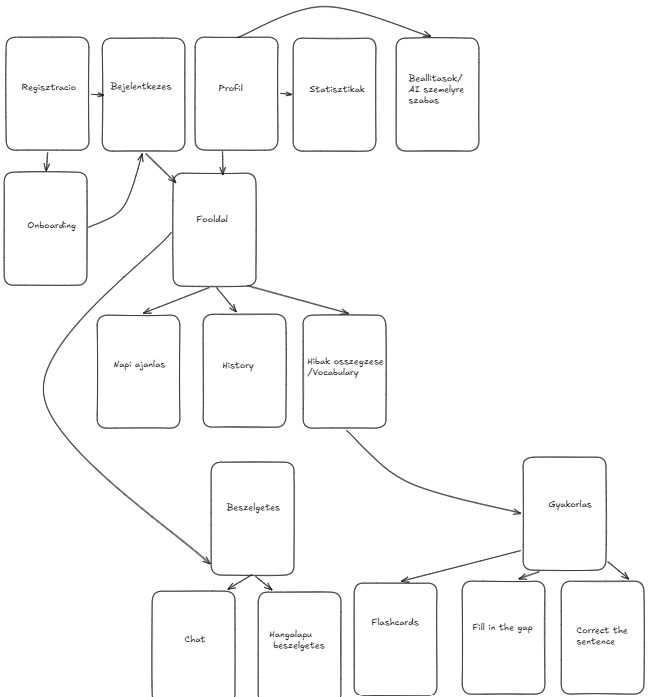
\includegraphics[width=0.8\linewidth]{images/fft.png}
    \caption{Felhasználói felület terv}
    \label{fig:fft}
\end{figure}

A felhasználói felületet tervezéséhez egy egyszerű digitális eszközt használtam. Mivel első sorban nem a felhasználói felület volt számomra a szempont, így inkább egy egyszerűbb tervet készítettem az Excalidraw \cite{excalidraw} alkalmazás használatával. Az alkalmazás fejlesztésénél ezeket vettem elő, ezek biztosították az irányt, amerre haladt a projekt. Néhol újabb dolgokat is beillesztettem fejlesztés közben, nem ragaszkodtam a kezdetleges terveimhez mindig.

A felület tervezésénél nem volt pontos irány, hogy merre rakjuk a gombokat, vagy milyen színeket használjunk, inkább egy átfogó képet szerettem volna kapni az alkalmazásról. Arra fektettem a hangsúlyt a tervben, hogy milyen oldalak, képernyők legyenek az applikációban és a többi részével fejlesztés közben foglalkoztam.

A \ref{fig:fft} ábrán látható a kezdetleges terv, amelyet még az elején a tervezési fázisban készítettem. Itt látható 17 darab képernyő terv és a nyilak jelölik az azok közötti kapcsolatokat. Mára elmondható, hogy a többsége ezeknek a terveknek megvalósult, és hasonlóan sikerült elkészíteni a kapcsolatokat is, mint ahogyan az ábrán látható. Így elmondható, hogy ez a tervezés mindenképpen megalapozta az elkészítés folyamatát.

Ez a tervezés nem csak a felhasználói felület elkészítésében volt hasznomra, hanem a teljes fejlesztés során. Mivel itt a nyilak segítségével megtekinthető a teljes flow, így nem csak a frontend fejlesztésnél, hanem a backend elkészítésénél is rálátást nyertem arra, hogy melyik feature mi után következzen.


\section{Verziókövetés}

A verziókövetés tekintetében a Github volt számomra egy elengedhetetlen választás. Ide mentettem minden elkészített featuret. Fontosnak éreztem a verziókövető rendszer használatát, ugyanis egy összetett rendszerről beszélünk, amelyben a működő komponenseket jó ha eltároljuk valahol és bármi elakadásnál vissza tudjuk húzni a működő verziót. Ez látható a  \ref{fig:github} ábrán. \cite{gitVersionControl}

Egy repository segítségével kezeltem a projektet, amelyben három nagy komponens szerepel: a backend, frontend és az ai service. 

\begin{figure}[ht]
    \centering
    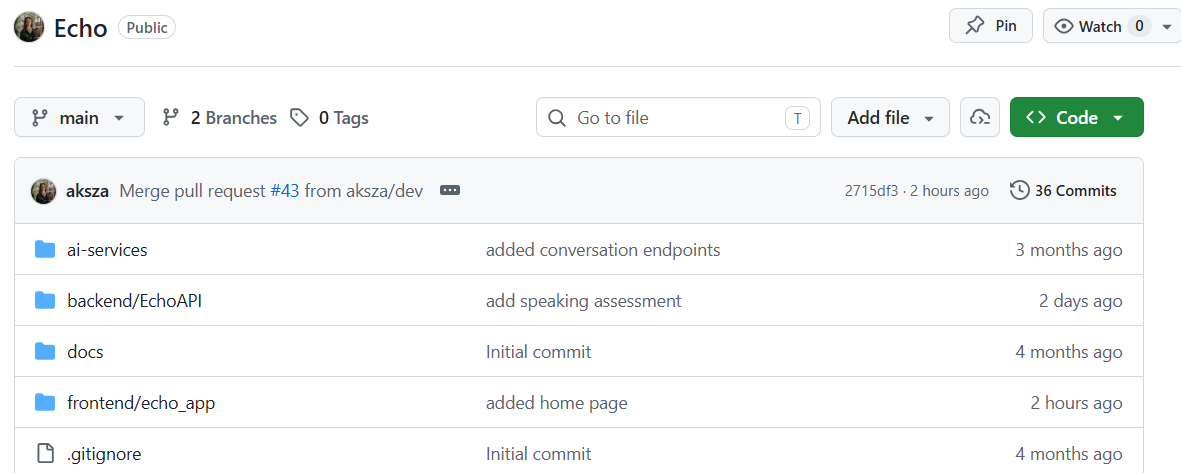
\includegraphics[width=0.9\linewidth]{images/git.png}
    \caption{Verziókövető rendszer}
    \label{fig:github}
\end{figure}

A hatékony programozáshoz készítettem egy branchet is, hogy a main branch tisztán maradhasson mindig, és a csak a működő feature komponensek legyenek itt, ne a félkészek. A dev branchen fejlesztettem mindent. Itt több commit is volt készítve minden featurehöz. Amikor sikerült elkészíteni egyet, pull request lett nyitva, itt mégegyszer megvizsgáltam a kódot, ha találok benne hibát. Amikor jónak tűnt, máris befésültem a mainre.Ezzel a megközelítéssel könnyedén és tisztán ment a fejlesztés. A branch ábrája a \ref{fig:branch} megtekinthető.


\begin{figure}[ht]
    \centering
    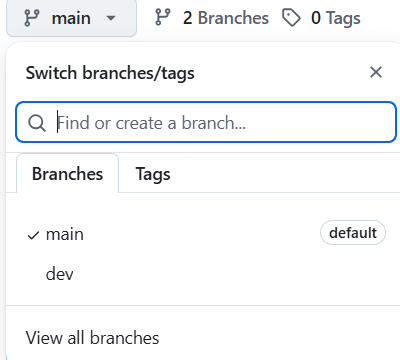
\includegraphics[width=0.4\linewidth]{images/branch.png}
    \caption{Branch-ek}
    \label{fig:branch}
\end{figure}

\section{Projektmenedzsment}

Próbáltam úgy megoldani a projektmenedzsmentet is, hogy azonos platformon legyen a verziókövetőnkkel. Így esett arra a választás, hogy a Github issues menüpontját használjam. \cite{githubIssues} Ez arról szól, hogy minden feature számára nyitok egy issue-t. Az issue-k tartalmazhatnak subissue-kat is, ha túl nagy issue jött létre. 

Ez számomra azért volt a legkézenfekvőbb, mivel egy platformon elérhetem a kész kódot, a feature terveket és pull request formájában a már kész, elfogadásra váró feature-öket. 

A flow az volt, hogy a tervezés résznél megírtam itt, issue formájában minden egyes feature-t, amelyet le kell implementálni. Ekkor meg lehetett itt adni, hogy ki kell elkészítse ezt - ez nagyobb csapat esetében nagyon hasznos lehet, de nálam értelemszerűen én voltam megjelölve itt. Ezután labelt, milestone-t is lehetett hozzáadni, viszont én az egyszerűség kedvéért ezeket a részleteket hanyagoltam. Miután elkészült a tervezés részben az összes issue, kezdődött a fejlesztés. Kiválasztott feature-t leimplementáltam, ezután pedig pull requestet nyitottam. Itt méginkább bebizonyosodott, hogy jó választás volt az, hogy ugyanazon a platformon verziózok és menedzselem a projektet is, ugyanis van egy olyan funkció, hogy a pull request leírásában ha hivatkozunk az adott issue-ra, akkor a pull request merge végrehajtása után automatikusan lezárja az issue-t. Így nem kellett manuálisan lezárnom minden elkészített feature-höz tartozó issue-t.

Az Github oldalán pedig bármikor megtekinthetőek voltak a nyitott vagy már lezárt issue-k. Ezeket bármikor újra lehetett nyitni, vagy akár a nyitottakat lezárni, duplikáltnak jelölni. Úgy gondolom, hogy ez egy olyan projekthez, amit egy személy készít, bőven elegendő projektmenedzsment eszköznek, mivel minden szükséges kellék megvan benne.

\newpage

\begin{figure}[ht]
    \centering
    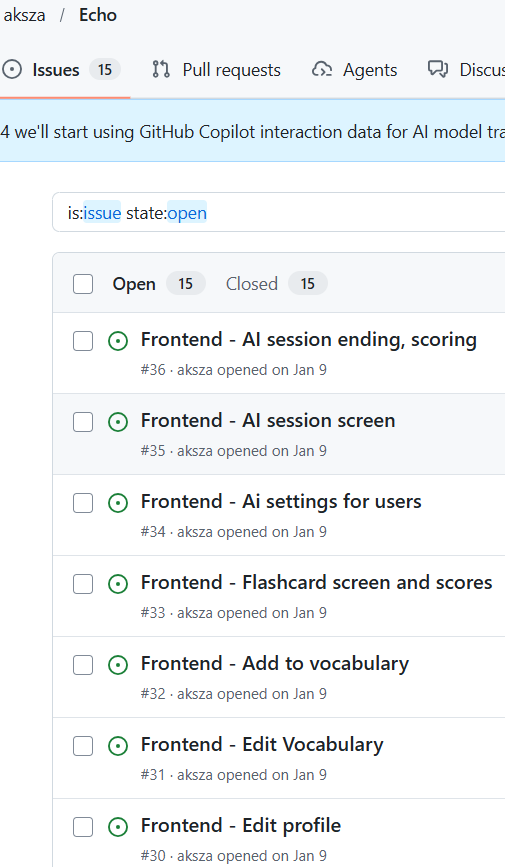
\includegraphics[width=0.5\linewidth]{images/issues.png}
    \caption{Projektmenedzsment}
    \label{fig:projectmanagement}
\end{figure}
	%----------------------------------------------------------------------------
\chapter{Megvalósítás}
%----------------------------------------------------------------------------

\section{Az alkalmazás architektúrája}
Az alkalmazás fejlesztése során fontos szempont volt egy jól struktúrált, könnyen bővíthető és karbantartható architektúra létrehozása. A rendszert három fő komponensből építettem fel: frontend réteg, backend réteg és AI service réteg. Ezek a komponensek mind egymástól elkülönítve működnek, kommunikációjuk HTTP alapú API hívásokon keresztül történik.



\section{Frontend megvalósítása}

Az alkalmazás kliensoldali része Flutter keretrendszer használatával készült. \cite{flutter} Ez lehetőséget biztosít modern, platformfüggetlen mobil vagy akár web és desktop alkalmazások fejlesztésére. A Flutter előnye nem más, mint hogy egyetlen kódbázisból több platformra is készíthető alkalmazás. Az Echo alkalmazásban a frontend réteg biztosítja a kapcsolatot a felhasználó és a rendszer többi komponense között, ezen keresztül történik minden fontos funkció elérése, mint a regisztráció, beszélgetés, gyakorlás, hibák és szókincs megtekintése.

A projekt felépítésénél első számú szempont az átláthatóság volt, ezért a fájlokat különböző mappákba csoportosítottuk, funkcionális egységek szerint elrendezve. A \textit{lib} mappában három fontos rész különíthető el: \textit{core}, \textit{features}, \textit{shared} mappa. Ez a szerkezett hozzájárult ahhoz, hogy az alkalmazás részei jól elkülönüljenek, ugyanakkor könnyen bővíthetők legyenek újabb funkcionalitásokkal.

A \textit{core} mappa tartalmazza az egész alakalmazás működéséhez szükséges elemeket. Ide tartoznak a konstans értékek, globális providerek, téma beállítások. A hálózati kommunikáció megvalósításához Dio csomagot  \cite{dio} használtam, amellyel HTTP kéréseket tudtunk küldeni a backend felé. Az API végpontok elérhetősége .env fájlban van eltárolva flutter dotenv csomag segítségével. \cite{flutterdotenv}

A \textit{features} mappa tartalmazza az alkalmazás fő funkcióit. Minden feature külön mappába került. Ez a feature alapú felépítés nagyon hasznos, mivel minden funckionalitás saját egységként kezelhető. A fejlesztés során nagyon megkönnyíti így a dologt, mivel könnyebben átlátható az, hogy melyik működéshez melyik fájl tartozik.

Például, a \textit{conversation} modul külön \textit{data} és \textit{presentation} rétegre oszlik. A \textit{data} réteg az API kommunikációhoz és adatmodellekhez kapcsolódó fájlokat tartalmazza. Ezek felelősek a backenddel való kommunikációért, mint például az üzenetek kezeléséért, valamint hangalapú beszélgetések válaszainak feldolgozásáért. A \textit{presentation} réteg viszont a felhasználói felülethez kapcsolódó komponenseket tartalmazza.  

Állapotkezelés szempontjából a \textit{flutter riverpod} \cite{riverpod} csomagot vettem használatba. Ez a csomag hozzájárul ahhoz, hogy az alkalmazás különböző részei könnyen elérjék és frissítsék a szükséges adatokat, például a bejelentkezett felhasználó adatait, a beszélgetések állapotát vagy a betöltési folyamatokat. Ennek az előnye az, hogy jól illeszkedik a moduláris felépítéshez, és hozzájárul az állapotkezeléshez.

Az alkalmazásban az egyik fontos funkcionalitás a hangalapú kommunikáció. Erre három különböző csomagot használtam fel. A \textit{record} segítségével a felhasználó hangot tud rögzíteni, amelyet később továbbíthatják a backend felé, feldolgozásra. Az \textit{audioplayers} csomag a hangválaszok lejátszására szolgálnak, míg a \textit{path provider} a fájlok ideiglenes vagy helyi tárolásában nyújt segítséget. \cite{record,audioplayers,pathprovider}

Mégegy fontos mappa a \textit{shared} mappa. Itt olyan újrafelhasználható elemeket tárolunk, amelyeket több képernyőn is megjeleníthetünk. Ide tartoznak a közös widgetek, amelyekkel egységessé varázsoljuk a felületet. Ennek a mappának segítségével csökkentettem a kódismétlést és megkönnyítette a későbbi módosításokat.

Összességében a frontend megvalósítása során egy jól struktúrált, funkcionalitás alapú Flutter alkalmazás jött létre, amely jól kezelhető, képes kommunikálni megfelelően az APIval, valamint támogatni a szöveges és hangalapú nyelvtanulási folyamatokat.

\newpage

\section{Backend megvalósítása}

Az alkalmazás szerveroldali komponensét ASP.NET Core Web API hasnzálatával készítettem. \cite{aspnetcore} Itt valósul meg a felhasználói hitelesítés, üzleti logika, adatbázissal való kommunikáció, illetve a mesterséges intelligenciát biztosító szolgáltatásokkal való kapcsolat fenntartása. A fejlesztés során fontos szempont volt a kód átláthatósága, karbantarthatósága, így esett a választás a Clean architektúrára. \cite{martin2017cleanarchitecture}

A projekt négy fő rétegre bontható: API, Application, Core és Infrastructure. Ezek a rétegek mind elkülönült felelősséggel rendelkeznek, kevés függőséggel, így egyszerű, hosszútávú fejlesztéséhez járul hozzá.

\begin{itemize}
    \item \textbf{API réteg:}
    
    Az API réteg felelős a kliens alkalmazás és a backend közötti kapcsolat létesítésében. Itt HTTP kérések segítségével kommunikálhatnak egymással.

    Különböző mappák találhatóak ebben a rétegben, mindegyiknek különböző, de nagyon fontos szerepe van a projekben.

    A Controller mappában különböző végpontok tárolódnak el. Ez a mappa ezeknek a végpontok kezeléséért, tárolásáért, rendszerezéséért felelős. Többek között ezek a végpontok biztosítják a felhasználói hitelesítést, beszélgetés kezelést, beállításokat, és még sok egyebet.

    A DTO mappában szerepelnek azok az osztályok, amelyek az adatátvitelt szolgálják a kliens és szerver között. Ezek az osztályok nagyon fontos szerepet játszanak a projektben, mivel hozzájárulnak ahhoz, hogy csak a szükséges adatokat továbbítsuk a kliens számára. Ezáltal növeljük a rendszer biztonságát és rugalmasságát.

    A Mappings mappa tartalmazza az AutoMapper  \cite{automapper} konfigurációit. Itt automatikusan átalakítjuk az entitásokat DTO objektumokká és ugyanúgy fordítva. Ez olyan szempontból hasznos, hogy leredukálja a manuális konvertálások számát, egyszerűsíti a fejlesztést, így időt spórol ugyanakkor van egy központi helye ezeknek az átalakításoknak.

    Van egy Middleware \cite{aspnetcoreMiddleware} is a rendszerben, amelyben a globális hibakezelést valósítottam meg. Ennek feladata, hogy központilag kezelje az előforduló hibákat és egységes formátumú válaszokat küldjön a kliens számára.

    \item \textbf{Application réteg}

    Ez a réteg tartalmazza az alkalmazás üzleti logikáját. Itt olyan szolgáltatásokkal találkozhatunk, amelyek a különböző folyamatok működését valósítják meg.

    Itt történik például a felhasználók kezelése, hibák eltárolása, AI szolgáltatásokkal kapcsolatos implementációk. Itt nem szabad adatbázis specifikus megvalósításokat tárolni, kizárólag üzleti logikát, és interfészek segítségével valósul meg a kommunikáció a külső komponensekkel.

    \item \textbf{Core réteg}

    Ez az a réteg, amely a rendszer legbelső része. Itt vannak az alkalmazás alapvető elemei, domain logikái.

    Az Entities mappa az adatbázis entitásait tárolja, ezek az üzleti objektumok. Ezeknek segítségével és az Entity Framework segítségével jöttek létre code first módon az adatbázis táblái.

    Az Enums mappában tároljuk a felsorolásokat, ennek segítségével egységes kezelési módot alakítunk ki az különböző állapotok és kategóriák között.

    Az Interfaces mappa egy nagyon fontos hely, mivel ezek határozzák meg a szolgáltatások működését. A dependency injection ennek segítségével valósul meg, amely lehetővé teszi azt implementációk egyszerű cseréjét és a rendszer jobb tesztelhetőségét. \cite{dotnetDI}

    \item \textbf{Infrastructure réteg}

    Itt a külső szolgáltatások és adatbázis eléréseket valósítom meg.

    A Data mappa szolgál az adatbázis kapcsolat konfigurációjában, a DbContext osztály pedig a táblák beállításait és a kapcsolatok kezeléseit biztosítja.

    A Repositories mappa olyan osztályokat tartalmaz, amelyek az adatbázisműveletek implementációit tartalmazza. Ezek az osztályok lekérdezéséért, módosításáért, létrehozásáért és törléséért felelősek. A repository minta lett itt alkalmazva, amely elkülöníti az adatkezelést az üzleti logikától.

    A Services mappában olyan szolgáltatások vannak, amelyek külső rendszerekkel kommunikálnak. Itt leginkább a repository osztályokat hívjuk, illetve itt valósul meg az AI szolgáltatások hívása is.

    Nem utolsó sorban a Utils mappát is megtalálhatjuk itt, amely különböző segédosztályokat tartalmaz, amelyeket bárhol a programban felhasználhatunk.

    \item \textbf{Program konfiguráció}

    A rendszer indulásakor a Program.cs fájl központi szerepet játszik. Ez végzi el az alkalmazás konfigurációját. Itt állítódik be az adatbázis kapcsolat, dependency injection konfigurálása, jwt hitelesítés beállítása, middlewarek regisztrációja. \cite{jwt}
\end{itemize}

% \newpage

\section{AI service megvalósítása}

A mesterséges intelligenciához kapcsolodó funkciók külön Python alapú mikroszolgáltatásokként lettek megvalósítva. \cite{fowlerMicroservices} Ez a felépítés nagyon előnyös, mivel így elkülönül a .NET backend az AI funkcióktól. Ezzel külön fejleszthetővé válik minden rész, szükség esetén könnyen módosítani lehet minden részt, vagy akár cserélni is. 

Az AI réteg három fő szolgáltatásból áll össze: beszédfelismeréshez a Whisper service járul hozzá, a nyelni modell a Phi3 service , a szövegfelolvasást pedig a Piper service végzi. 

Mindhárom szerviz hasonló projektstruktúrával rendelkezik. Mindhárom mappában külön mappa van az API útvonalaknak, konfigurációs fájloknak, adatmodelleknek és a logikát tartalmazó osztályoknak. Az api mappa endpointokat tartalmaz, a core konfigurációkat, models a kérés és válaszmodelleket, és a service az adott AI funkció tényleges megvalósítását.

Elsőszámú AI service a Whisper, amely azért felelős, hogy a beszédet szöveggé alakítsa. Itt faster whispert használtam, amely egy gyors változata a modellnek. \cite{whisper,fasterwhisper} Az alkalmazásban ez lesz az a komponens, ami elsőként hívódik meg, amikor a felhasználó a mesterséges intelligenciához beszél, ez pedig szöveges formátummá fogja átalakítani a következő lépéshez.

A Phi3 service a nyelvi intelligenciát biztosítja. Ez beszélgetésre és utasításkövetésre optimalizált nyelvi modell. Feladata az, hogy a megadott szövegre utasítás szerinti válaszokat generáljon, felismerje és kijavítsa a nyelvi hibákat a visszaadott szövegben. \cite{phi3}

A Piper service a harmadik fázishoz járul hozzá a válaszadásban, amikor a szöveges választ, amelyet a Phi3 generált, beszéddé alakítja. Ez azért fontos, mert egy valós beszélgetést szerettem volna leszimulálni, hogy a felhasználó könnyebben memorizálja és hozzászokjon, milyen a valódi kommunikáció. \cite{piper}

A backend API HTTP kéréseken keresztül kommunikál ezekkel a mikroszolgáltatásokkal.
    %%----------------------------------------------------------------------------
\chapter{Felhasználói felület}
%----------------------------------------------------------------------------

Felhasználói felületet tekintve, igyekeztem egy letisztult, nem túl zsúfolt, egyszerű és átlátható felületet biztosítani. Az alkalmazás meghatározó színe a narancssárga. A DineEase alkalmazásban két szerepkörbe tartozó felhasználó létezik: étterem és átlag felhasználó. Ezeknek két különböző felület jött létre, viszont egy dolog megegyezik, a bejelentkezés és regisztráció képernyők.


\section{Belépés és regisztráció}

Ahogy megnyitja az alkalmazást a felhasználó, egy splash screen megjelenése után, ha nem volt előzőleg bejelentkezve még, vagy lejárt a bejelentkezési ideje (tokenje), következik az a képernyő, ahol kiválaszthatja, hogy bejelentkezni szeretne vagy új fiókot szeretne létrehozni.


\begin{figure}[ht]
    \centering
    \includegraphics[width=0.32\linewidth]{Diplomadolgozat//images/bej.png}
    \caption{Bejelentkezés oldal}
    \label{fig:bej}
\end{figure}

\newpage


A Login gombra kattintva, elvezeti a bejelentkezéshez a felhasználót, ahol megadhatja adatait. Ha még nincs fiókja, átnavigálhat a Register now szövegre kattintva a regisztrációs felületre. Itt bármelyik szerepkörbe tartozó felhasználó be tud jelentkezni, ugyanis felismeri az alkalmazás, hogy milyen típusú felhasználó szeretne bejelentkezni. Ez látható a \ref{fig:bej} ábrán.

A Sign up gombot választva a regisztrációs oldallal találkozik a felhasználó. Itt kiválaszthatja, milyen szerepkörbe tartozó fiókot szeretne létrehozni, és aszerint tölti ki a szükséges adatokkal a mezőket. A mezők ellenőzik, hogy megfelelő formátumú adatot adott-e meg a regisztráló. Természetesen itt is van olyan opció, hogy átlépjenek a bejelentkezéshez, egy szövegre kattintva. A regisztrációs oldalak a \ref{fig:reg} ábrán láthatóak 

\begin{figure}[h]
    \centering
    \subfigure{
        \includegraphics[width=0.35\textwidth]{Diplomadolgozat//images/reg1.png}%
        \label{fig:reg1}%
    }
    \subfigure{
        \includegraphics[width=0.35\textwidth]{Diplomadolgozat//images/reg2.png}%
        \label{fig:reg2}
    }
    \caption{Regisztrációs oldalak}
    \label{fig:reg}
\end{figure}

\section{Felhasználó}

A \ref{fig:foryou} ábrán észrevehető, hogy egy navigációs sáv segítségével lehet váltogatni a négy oldal között: \textit{For You, Restaurants, Events, Restaurants for Events}. Itt használatba vehető a \textit{keresés} funkció is, illetve az ember ikonra kattintva a felhasználó a \textit{profil} oldalára is navigálhat.

\subsection{For you oldal}

A bejelentkezett felhasználó először a \textit{For You} nevű oldallal találkozhat, amelyet a \ref{fig:foryou} ábrán lehet látni. Itt ajánlásokkal találkozhat a felhasználó, négy szekcióra felosztva. A \textit{Trending} címszó alatt jelenik meg az a három étterem, amely az utóbbi hét napban a legtöbb foglalással rendelkezett. A \textit{You may also like} címszó alatt jelenik meg a három legnagyobb értékeléssel rendelkező étterem. A \textit{Recommended events} alatt olyan eseményeket ajánl az alkalmazás a felhasználónak, amelyeket olyan éttermek szerveznek, amiket kedvencnek jelölt be a felhasználó, ha nincs kedvence bejelölve, akkor egyszerűen néhány random eseményt ajánl. A \textit{Did you like} címszó nem mindenkinek jelenik meg, itt olyan éttermek láthatóak, amelyeket már meglátogatott a felhasználó, azaz a foglalásai szerint vannak listázva. 

Az éttermek megjelenítésénél látható egy \textit{kép}, a \textit{neve}, \textit{értékelése} és egy szív alakú ikon, amely megnyomásával lehet az adott éttermet \textit{kedvenc}nek megjelölni, vagy épp kitörölni a kedvencek közül.

\begin{figure}[h]
    \centering
    \includegraphics[width=0.4\linewidth]{Diplomadolgozat//images/foryou.png}
    \caption{For you oldal}
    \label{fig:foryou}
\end{figure}

\subsection{Keresés}

A \ref{fig:foryou} ábrán látható felül a kereső, ahol lehetőség van rákeresni éttermekre és eseményekre a beírt karakterek alapján. A kereső az éttermek és események nevében és leírásukban keresi a karaktereket és küldi vissza azok listáját.


\subsection{Restaurant és Event oldal}

A \ref{fig:resev} ábrán látható a Restaurant és Event oldal, ahol ki van listázva az összes étterem és az összes elkövetkező esemény, amelyeket szerveznek az éttermekben. Ugyanígy néz ki a Restaurants for Events oldal is, ahol azok az éttermek vannak kilistázva, ahol nagyobb eseményeket lehet szervezni. A Restaurants oldalnak a jobb felső sarkában található egy ikon, amely segítségével szűrhetjük különböző tulajdonság szerint az éttermeket.


\begin{figure}[h]
    \centering
    \subfigure{
        \includegraphics[width=0.4\textwidth]{Diplomadolgozat//images/res.png}%
        \label{fig:res}%
    }
    \subfigure{
        \includegraphics[width=0.4\textwidth]{Diplomadolgozat//images/ev.png}%
        \label{fig:ev}
    }
    \caption{Restaurant és Event oldalak}
    \label{fig:resev}
\end{figure}

\newpage

\subsection{Éttermekhez és eseményekhez kapcsolódó funkciók}

Ha kiválaszt egy éttermet, megtekintheti annak részletes információit, ez látható a \ref{fig:details} ábrán. Itt több funkció is elérhető. A szív alakú ikonra kattintva \textit{kedvencnek jelölheti} be az éttermet. A Rating címszó alatt \textit{értékelheti} az éttermet, vagy törölheti értékelését a felhasználó. \textit{Visszajelzést} is írhat az étteremről a felhasználó, vagy épp törölheti is a saját megjegyzését, és megtekintheti itt másokét is. A Show menu gomb lenyomásával megtekinthető az étterem által kínált menüsor.

Az események is hasonlóképpen jelennek meg, ott csak a részleteit lehet megtekinteni és ilyen funkcionalitásokkal nem rendelkeznek, viszont ott is megjelenik a Reserve a table gomb, amellyel asztalt lehet foglalni az esemény dátumára. 


\begin{figure}[h]
    \centering
    \subfigure{
        \includegraphics[width=0.4\textwidth]{Diplomadolgozat//images/details1.png}%
        \label{fig:det1}%
    }
    \subfigure{
        \includegraphics[width=0.4\textwidth]{Diplomadolgozat//images/details2.png}%
        \label{fig:det2}
    }
    \caption{Étterem részleteinek oldala}
    \label{fig:details}
\end{figure}

\newpage

\subsection{Foglalás és meeting programálás}

Mivel két fajta étterem kategóriát különböztetünk meg az alkalmazásban, így két különböző funkcionalitást is lehet elérni. 

A Restaurant for Event kategóriából kiválasztott éttermekbe meetinget lehet szervezni, ez a \ref{fig:foglmeet} ábrának a jobb oldalán látható, ahogyan különböző adatok megadásával egy személyes meetinget szervez a részletek megbeszélésére az étterem tulajdonosával. 

A Restaurants kategóriából választott étterembe foglalást lehet letenni, ami a \ref{fig:foglmeet} ábra bal oldalán tekinthető meg. Itt lehet a Menu gombra kattintva előrendelni az ételt a foglaláshoz, ezek a megrendelt ételek megjelennek a foglalás oldalán is, ahol az összeget is írja, amennyit fizetnie kell majd, viszont ha úgy dönt, hogy mégsem szeretné azt a menüt választani, kitörölheti egy gomb lenyomásával.


\begin{figure}[h]
    \centering
    \subfigure{
        \includegraphics[width=0.41\textwidth]{Diplomadolgozat//images/fogl.png}%
        \label{fig:fogl}%
    }
    \subfigure{
        \includegraphics[width=0.4\textwidth]{Diplomadolgozat//images/meet.png}%
        \label{fig:meet}
    }
    \caption{Foglalás és meeting programálás oldalak}
    \label{fig:foglmeet}
\end{figure}

\newpage

\subsection{Profil oldal}

A \ref{fig:foryou} ábrán látható a jobb felső sarokban egy profil ikon, erre kattintva érhető el a Profil oldal, amelyen a felhasználóval kapcsolatos információk érehetőek el, ezeknek a választéka a \ref{fig:profil} ábrán látható.

Az \textit{Edit profile} gombra kattintva a felhasználó a saját adatait szerkesztheti.

A \textit{Favorits} gombra kattintva megjelenik az összes étterem listája, amelyet a felhasználó kedvencnek jelölt, itt ki is lehet őket törölni a kedvencek közül.

A \textit{Reservations} gombbal megtekintheti azokat a foglalásait, amelyekre kapott választ az éttermektől, hogy elfogadták őket vagy sem. Itt elsősorban az elkövetkező foglalások jelennek meg, utána pedig egy History a régi foglalások listájával.

\begin{figure}[ht]
    \centering
    \includegraphics[width=0.4\linewidth]{Diplomadolgozat//images/profil.png}
    \caption{Profil oldal}
    \label{fig:profil}
\end{figure}

\newpage

\section{Étterem}

Az éttermek mivel két kategóriába sorolhatók, így néhány eltérő funkció is látható, de összességében nagyon hasonlóak.

\subsection{Foglalás és Meeting oldal}

A \ref{fig:rfoglalas} ábrán látható, hogyan jelennek meg az étterem foglalásai . Itt az elfogadott foglalásai láthatóak. Három különféle nézetben tudja megtekinteni ezeket: havi, heti és napi. A napi nézetben, ha rákattint egy adott foglalásra, akkor láthatja a foglalás részleteit. Ha rendelt is a foglaló személy, akkor a \textit{See orders} gombra kattintva meg lehet tekinteni a rendeléseit is. Hasonlóképpen jelennek meg a meetingek is.

\begin{figure}[h]
    \centering
    \subfigure{
        \includegraphics[width=0.4\textwidth]{Diplomadolgozat//images/rres1.png}%
        \label{fig:foglalas1}
    }
    \hspace{0.05\textwidth}
    \subfigure{
        \includegraphics[width=0.4\textwidth]{Diplomadolgozat//images/rres2.png}
        \label{fig:foglalas2}
    }
    \caption{Foglalások megtekintése}
    \label{fig:rfoglalas}
\end{figure}

\newpage

\subsection{Waitinglist oldal}

A waitinglist-be a válaszra váró foglalások és meetingek kerülnek be. Itt átnézheti őket az étterem és elfogadhatja vagy éppen elutasíthatja őket az Accept és Reject gombokkal. Ez látható a \ref{fig:rwaiting} ábrán.

\begin{figure}[ht]
    \centering
    \includegraphics[width=0.4\linewidth]{Diplomadolgozat//images/rwaiting.png}
    \caption{Waitinglist oldal}
    \label{fig:rwaiting}
\end{figure}

\newpage

\subsection{Your Events oldal}

Az eseményeket, amelyeket már megszerveztek az étteremben vagy éppen szerveznek, a menüsor \textit{Your events} gombjára kattintva érheti el. Itt a régi eseményekre kattintva megtekinthetőek a részleteik, az elkövetkező eseményekre kattintva pedig szerkeszteni is lehet őket. Ezen az oldalon lehet új eseményeket is meghirdetni a plusz gombra kattintva. Ez látható a \ref{fig:revent} ábrán.

\begin{figure}[ht]
    \centering
    \includegraphics[width=0.4\linewidth]{Diplomadolgozat//images/revent.png}
    \caption{Your events oldal}
    \label{fig:revent}
\end{figure}


\subsection{Your Menu oldal}

Az étteremnek lehetősége van menüket is hozzáadni, ehhez létrejött az az oldal, amelyet a menüsor \textit{Your Menu} gombjára kattintva érhet el. Itt hozzáadhat új menüket és szerkesztheti a meglévőket, illetve törölheti is őket.

\newpage

\subsection{Restaurant oldal}

Az étterem a saját információit szerkesztheti a \textit{Restaurant} gombra kattintva a menüből. Ez az oldal látható a \ref{fig:rprofil} ábrán. Itt megadhat frissebb információkat az étteremről és képeket tölthet fel vagy törölhet.

\begin{figure}[h]
    \centering
    \subfigure{
        \includegraphics[width=0.4\textwidth]{Diplomadolgozat//images/rprof.png}%
        \label{fig:rprof1}
    }
    \hspace{0.05\textwidth}
    \subfigure{
        \includegraphics[width=0.4\textwidth]{Diplomadolgozat//images/rprof2.png}
        \label{fig:rprof2}
    }
    \caption{Étterem profil oldal}
    \label{fig:rprofil}
\end{figure}

\newpage

\subsection{Statistics oldal}

Az étteremről készül néhány statisztikai mérés is, ami ezen az oldalon érhető el. Ha a \textit{for event} kategóriába sorolandó étterem információit vizsgáljuk, akkor ezen az oldalon jelenik meg az átlag napi meetingek statisztikája, az elmúlt hónap meetingjeinek statisztikája, egy statisztika arról, hogy melyik órában a legforgalmasabb az étterem, és az elmúlt öt hét eseményeinek száma oszlopdiagrammal. Az átlag éttermek annyiba különböznek ettől, hogy mérve van a rendelések száma is foglalásonként, illetve az előzőekben felsoroltakban nem a meetinget, hanem a foglalásokat méri. Ugyanakkor itt látható az étterem értékelése is és megtekinthetőek a visszajelzések is. Ezeket a visszajelzéseket itt törölni is lehet, ha nem tetszene a tartalma.

\begin{figure}[h]
    \centering
    \subfigure{
        \includegraphics[width=0.4\textwidth]{Diplomadolgozat//images/rstat.png}%
        \label{fig:stat1}
    }
    \hspace{0.05\textwidth}
    \subfigure{
        \includegraphics[width=0.4\textwidth]{Diplomadolgozat//images/rstat2.png}
        \label{fig:stat2}
    }
    \caption{Statisztikák oldal}
    \label{fig:stat}
\end{figure}
    %----------------------------------------------------------------------------
\chapter{Kutatási terv és értékelési módszertan}
%----------------------------------------------------------------------------

A dolgozat gyakorlati részében az kerül vizsgálatra, hogy milyen az elkészített AI alapú szoftver mennyire járul hozzá a tanulók témaspecifikus szókincsfejlődéséhez, beszédkészségéhez, hibafelismeréséhez és tanulási motivációjához a hagyományos tanítási módszerhez viszonyítva. Mindezt egy rövidtávú kontrollcsoportos pilot vizsgálat során derítjük ki.\cite{vanTeijlingen2001pilot}

A vizsgálat egy 40 perces angol nyelvű tanóra keretében valósul meg. Ennek témája a technológiahasználat és az online biztonság, amelyben kitérünk a kártékony szoftverek típusaira is. A tananyag sok új, fontos fogalmat dolgoz fel, mint például: virus, worm, trojan horse, ransomware, personal information, password, suspicious link. A választott téma alkalmas a szókincsfejlesztés, a szövegértés és beszédalapú gyakorlás vizsgálatára is.

A kutatásban összesen 16 tanuló vesz részt, akik egy magántanár diákjai. A tanulók életkora 12 és 16 év között mozog, nyelvi szintjük pedig A2 és B2 közötti. A nemi eloszlás azonos, tehát 8 fiú és 8 lány van, minden csoportban 4-4 közülük. A résztvevők két 8 fős csoportra osztódnak, amiben vegyesen van gyengébb és erősebb szintű tanuló is. A kontrollcsoport hagyományos tanítási módszerrel dolgozza fel a témát, míg a kísérleti csoport AI alapú alkalmazás segítségével tanul.

Mivel a kutatásban kiskorú tanulók vesznek részt, az adatok kezelése anonim módon történik. A neveik nem jelennek meg eredményekben, sem adatbázisban, helyette K1-K8 kódokkal jelöljük őket, míg az AI alapú alkalmazást használó csoportot A1-A8 kóddal. 

A vizsgálatnak a mérésére használunk előtesztet, utótesztet \cite{campbell1963experimental}, beszédkészség mérést és kérdőívet. Az előteszt célja a tanulók kiindulási tudásszintjének mérése, míg az utóteszt a tanulási folyamat után elért eredmények mérésére szolgál. A beszédkészség vizsgálata rövid, irányított beszélgetések alapján történik, míg a kérdőív a tanulói élményt, motivációt és az alkalmazás használhatóságát méri.

\section{A kutatás célja}

A kutatás célja annak vizsgálata, hogy az AI alapú nyelvoktatás milyen szinten támogatja a beszédfejlesztést, szókincs gyarapítást, motivációt, a tanulók rövid távú tanulási eredményei megvizsgálásával, úgy hogy egy konkrét angol nyelvi témát dolgoznak fel. 

A kutatás, mivel két különböző módszert vizsgál, összehasonlító jellegű. Az egyik csoport hagyományosabb, tanári irányítással tanul, amelyben prezentáció, vocabulary feladat és beszélgetés az alapja a lecke elsajátításának. A másik csoport ugyanazt a témát boncolgatja, viszont az alkalmazás keretein belül. Itt a leckét elolvashatja, kijelölheti az ismeretlen kifejezéseket, beszélget az AI aszisztenssel a témáról, amely vizsgálja közben a hibáit, végül pedig a hibákat átismétli.

A kutatás rövidtávú vizsgálatként értelmezhető. Ennek megfelelően az eredmények célja nem általános érvényű következtetéseket von le, hanem annak előzetes vizsgálatára szolgál, hogy az alkalmazás alkalmas lehet oktatási környezetben, és milyen lehetőségeket nyújt a hagyományos módszerekhez képest.

\section{Kutatási kérdések és hipotézisek}

A kutatás során négy darab kérdés tevődik fel, amelyhez kapcsolódik négy hipotézisem.

A kérdések a következők:
\begin{quote}
\begin{enumerate}
    \item Milyen mértékben fejlődik a tanulók témaspecifikus angol szókincse az AI alapú alkalmazás használata után?
    \item Van-e különbség a hagyományos tanítási módszerrel és az AI alapú alkalmazással tanuló csoport eredményei között?
    \item Milyen hatással van az AI alapú alkalmazás használata a tanulók beszédkészségére egy adott témáról folytatott beszélgetés során?
    \item Hogyan értékelik a tanulók az AI alapú alkalmazás használhatóságát, érthetőségét, motiváló hatását?
\end{enumerate}
\end{quote}

A kutatási kérdésekre a következő hipotézisek fogalmazhatók meg:
\begin{quote}
\begin{enumerate}
    \item Az AI-alapú alkalmazást használó tanulók témaspecifikus szókincse fejlődik az előteszt és az utóteszt eredményei alapján.
    \item Az AI-alapú alkalmazást használó csoport fejlődése nagyobb mértékű lesz, mint a hagyományos módszerrel tanuló kontrollcsoporté.
    
    \item Az AI-alapú alkalmazást használó tanulók beszédkészsége javul az adott témáról folytatott irányított beszélgetés során.
    
    \item A tanulók pozitívan értékelik az AI-alapú alkalmazás használhatóságát, érthetőségét és motiváló hatását.
\end{enumerate}
\end{quote}

\section{A tanóra témája és menete}
A tanórák 40 percből állnak, amelyeken kétféleképpen fogjuk megtanítani a diákokat a technológiahasználatról, amelyben sok új kifejezést is tanulhatnak és a beszédkészségüket is növelhetik. Ebben a témában fogunk tesztelni.

A kontrollcsoport esetében az óra hagyományosan, tanári magyarázattal és prezentációval történik. Miután ez megvalósult, vocabulary feladatokat kezdenek oldani, utána pedig brainstorming résszel folytatják, amelyben a tanulók a témához kapcsolódó kérdésekre válaszolnak.

A kísérleti csoport ugyanazt a témát dolgozza fel, az applikáció segítségével. Az applikációban megtalálja ugyanazt a tananyagot szöveg formájában, amelyet meg is hallgathat. Itt kijelöli az ismeretlen kifejezéseket, amelyeket később tanulhat. Ezek után AI által vezetett beszélgetés történik, ahol a témáról beszélgetnek. Itt hibavizsgálat folyik a háttérben beszélgetés közben, és ezután a megállapított hibákat újra begyakorolhatja, és elsajátíthatja helyesen a kifejezéseket.

A két tanulási folyamat eltérő, de ugyanarra a tananyagra készíti fel a tanulókat. Ez lehetővé teszi, hogy egy adott téma tanulási módszerét vizsgáljuk.

\section{Mérőeszközök}
A kutatás során több mérőeszközt is használok, annak érdekében, hogy a tanulási eredményt több szempontból is megvizsgáljuk. Az értékelés kiterjed szókincsfejlődésre, beszédkészségre, tanulói motivációra is. Ennek megfelelően különböző méréseket veszek igénybe.

Elsősorban írásbeli tesztekkel mérek. Ez előteszt és utóteszt formájában valósul meg, \cite{campbell1963experimental} ahol a tanulók kiindulási tudásszintjének felmérése történik meg a tanóra előtt és a tanóra utáni megszerzett tudást is felméri. A feladatok között szerepel a szó-jelentés párosítás, mondatkiegészítés, rövid válaszok írása kérdésekre. 

A tanulói motiváció és élmény mérése kérdőív kitöltésével történik. A kérdőívben 1 és 5 között kell pontozni az állításokat, amelyek vizsgálják, hogy a tanulók mennyire találják hasznosnak, érdekesnek, motiválónak a tanulási módszert.

Az alkalmazással tanuló csoportoknál adatforrásként szolgál az alkalmazásban rögzített tanulási adatok, mint az ismeretlen szavak száma, vocabulary, helytelen mondatok. Ezek az adatok azt is lehetővé teszik, hogy vizsgáljuk, milyen mértékben használták az alkalmazás funkcióit.

\section{Adatelemzési módszerek}
Az adatok elemzése kvantitatív és kvalitatív szempontokkal történik. A kvantitatív elemzés méri, hogy a tanulók teljesítménye mennyire változik az előteszt és utóteszt között, és azt is hogy a kontrollcsoport és a kísérleti csoport eredményei között megfigyelhető lehet különbség vagy sem.

Elsőszámú mérés a leíró statisztikai mutatók kiszámítása. Itt kiszámoljuk az átlagot, szórást, minimum, maximum értékeket előteszt és utóteszt közötti fejlődésben. Ugyanez alkalmazható a beszédkészség felmérésében is, ahol az előtesztre és utótesztre is kap a tanártól pontot.

A csoportokon belüli fejlődés vizsgálatára páros t-próba alkalmazható, \cite{field2013statistics} ahol a tanulók előtesztjei és utótesztjeinek eredményét hasonlítjuk. Ezzel kimutatható, hogy az adott csoportban történt-e statisztikailag kimutatható fejlődés. A kontroll és a kísérleti csoportokat is összehasonlítom, független t-próbával, amely azt vizsgálja, hogy a két módszer között van-e jelentős fejlődési különbség.

A statisztikai szignifikancia mellett a hatásméretet is megmérem a Cohen-féle d értékkel. \cite{cohen1988statistical} Itt a két csoport közötti különbséget gyakorlati szempontból vizsgálom. Ez azért szükséges, mert kis minta esetén előfordul, hogy egy különbség nem tűnik statisztikailag szignifikánsnak, viszont pedagógiai vagy gyakorlati szempontból mégis figyelemreméltó tendenciát mutathat ki.

A kérdőíves válaszok elemzése leíró statisztikai módszerekkel történik. A kijelentéseket 1 és 5 között kell pontozzák, ezek alapján pedig az átlagértékből kiszámítható a motiváció, érdeklődés, használhatóság és elégedettség az alkalmazással szemben.

\section{Etikai szempontok}
A kutatás során kiemelt figyelmet szenteltem etikai szempontokra, mivel a vizsgálat során kiskorú résztvevőket mérünk fel. A részvétel önkéntes alapon történik, szülők is beleegyeztek és tájékoztatást kaptak a kutatás céljáról, adatok felhasználásáról és kezeléséről, illetve a tanár is beleegyezett, hogy az órái keretében vizsgáljak.

Az adatkezelés végig anonim módon történik. A tanulók nevei sem teszten, sem eredményekben nem szerepelnek. A résztvevők azonosítása kódokkal történik. Az így szerzett adatok kizárólag dolgozat kutatási céljára használható fel és nem alkalmas a tanulók személyes azonosítására.

A beszédkészség felmérésénél nem készülhet sem hangfelvétel, sem videófelvétel. A beszélgetés során a tanár az előre elkészített értékelési rubrika alapján közvetlenül a beszélgetés során rögzíti a pontszámokat. Ez a megoldás adatvédelmi szempontból lett alkalmazva.

A kutatás etikai szempontból fontos eleme az is, hogy az alkalmazás használata során keletkező adatok csak korlátozott célból kerüljenek felhasználásra. Az adatokat csak tanulási folyamat támogatását és kutatási elemzést szolgálják, harmadik fél számára semmi módon sem kerülhetnek továbbításra.
    %----------------------------------------------------------------------------
\chapter{Kutatási eredmények és kiértékelés}
%----------------------------------------------------------------------------

A dolgozat ezen részében egy rövid távú felmérés segítségével értékeljük ki a megvalósított rendszert. A vizsgálat célja az, hogy megértsük, milyen mértkben és módon támogatja az AI alapú alkalmazás használata a tanulási folyamatot, témaspecifikus szókincsfejlődést, beszédgyakorlést, valamint a tanulók motivációját egy hagyományos módszerhez képest.

A kuttás alatt 16 tanulót mértünk, 8 tanuló használta a hagyományos módszert, míg 8 tanuló az AI alapú alkalmazást. Az értékelés során előteszt, utóteszt, beszédkészség mérés került feldolgozásra. Az tesztek eredményeinek összehasonlítására leíró statisztikai elemzést végeztem, amely magában foglalja az átlagok, szórások és a különbségek vizsgálatát a két csoport között. Emellett a csoportokon belüli fejlődést párosított t-próbával értékeltem, hogy megállapítsam, van-e szignifikáns javulás a tanulók teljesítményében a tesztek között, illetve a két csoport közötti fejlődés különbséget független mintás t-próbával vizsgáltam.

Az mérés mivel rövid távú, nem ad nekünk teljes képet a használhatóságról és a hosszú távú hatásokról, hanem inkább az a célja hogy megvizsgáljuk vele, hogy működőképes-e az oktatási környezetben, és milyen tanulói visszajelzéseket kapunk a használat során.

\section{A vizsgálat lebonyolítása}

A vizsgálatban 16 tanuló vett részt, akik egy magántanár diákjai. 8 hagyományos oktatási módszerrel tanulta ugyanazt a témát, míg a másik 8 tanuló az alkalmazással tanulta.

A tanulási folyamat minden diáknak 40 percet vett igénybe. A tanóra témája a technológiahasználat volt, amely során a tanulók az online biztonságróé, kártékony szoftverekről és a digitális eszközök használatáról tanultak.

A kontrollcsoport tanulási folyamata egy hagyományosabb módszerrel zajlott, amely során a tanár prezentációt tartott a témáról, majd vocabulary feladatokkal és beszélgetéssel illetve brainstorminggal folytatták. A kísérleti csoport ezzel ellentétben az alkalmazásban olvasta el a lecke szövegét, vagy felolvastathatta az AI asszisztenssel is, illetve a szavakat is felolvastathatta vele, hogyha nem tudta a kiejtést. Ebben a szövegben kijelölhette az ismeretlen szavakat vagy kifejezéseket, amjd AI asszisztnssel beszélgetett a témában. A beszélgetés során az alkalmazásban tárolódtak a hibák, amelyeket beszélgetés után flashcardok segítségével vagy javításos feladatokkal gyakorolhattak.

A mérés mindkét csoport eseténben az óra elötti előtesztből, óra utáni utótesztből és a beszédkészség méréséből állt, miután kérdőívvel gyűjtöttük be a visszajelzéseket. Az előteszt segített megadni a kiindulási pontjukat a diákoknak, az utóteszt pedig a tanulás hatékonyságát mérte. Ezzel mértük a tanulók fejlősését, élményét, motivációját, és használhatóságát az alkalmazásnak.

\section{A csoportok előteszt eredményeinek összehasonlítása}

Az előteszt célja annak felmérése, hogy a kontrollcsoport és a kísérleti csoport tanulói milyen kiindulási szinttel rendelkeznek a tanulás megkezdése előtt. Ez azért nagyon fontos, mivel két tanulási módszer összehasonlításához elengedhetetlen szempont az, hogy mindkét csoport hasonló kiindulási ponttal rendelkezzen nagyjából.

Az előteszten 20 pontot lehetett elérni, ez a tanóra témájához kapcsolódó szókincset, fogalomértést vizsgálta. A feladatok között szerepelt a szó-jelentés párosítás, fill in the gap, valamint kérdés-válasz típusú feladatok. A két csoport eredményeit leíró statisztikai adatotait a~\ref{tab:eloteszt-leiro-stat} táblázat mutatja be.

\begin{table}[h!]
    \centering
    \begin{tabular}{lccc}
        \hline
        \textbf{Csoport} & \textbf{Létszám} & \textbf{Előteszt átlaga} & \textbf{Szórás} \\
        \hline
        Kontrollcsoport & 8 & 5.75 & 1.19 \\
        Kísérleti csoport & 8 & 5.62 & 2.17 \\
        \hline
    \end{tabular}
    \caption{Az előteszt eredményeinek leíró statisztikái csoportonként}
    \label{tab:eloteszt-leiro-stat}
\end{table}

A táblázat adatai alapján látható, hogy a két csoport előteszt eredményei közel hasonló eredményekkel rendelkeznek, a kontrollcsoport átlaga 5.75, míg a kísérleti csoport átlaga 5.62. Ez arra utal, hogy a tanulók hasonló szinttel rendelkeznek, így a két csoport összehasonlítható kiindulási tudásszinttel rendelkezik.

\begin{table}[h!]
    \centering
    \renewcommand{\arraystretch}{1.2}
    \begin{tabular}{p{4cm}cccc}
        \hline
        \textbf{Csoport} & \textbf{t érték} & \textbf{Szabadságfok} & \textbf{p-érték} & \textbf{Értelmezés} \\
        \hline
        Kontrollcsoport előteszt vs. kísérleti csoport előteszt & 0.13 & 14 & 0.896 & Nincs jelentős különbség \\
        \hline
    \end{tabular}
    \caption{Az előteszt t-próba eredményei a két csoport között}
    \label{tab:eloteszt-t-proba}
\end{table}

A \ref{tab:eloteszt-t-proba} táblázatban látható, hogy a függetelen mintás t-próba eredményei alapján nincs szignifikáns különbség a két csoport előteszt eredményei között. Az előteszt eredmények alapján tehát nem mutatható ki statisztikailag szignifikáns különbség a két csoport között. t(14)=0.13, p=0.896. Ez arra utal, hogy a kéy csoport hasonló kiindulási szinttel rendelkezik a vizsgálat kezdetén, így a összehasonlíthatónak tekinthetők.

\section{Előteszt és utóteszt eredményei csoporton belül}

A következő lépésben a csoportokon belüli fejlődést vizsgáltam meg. Mindkét csoport esetében összehasonlítottam az előteszt és utóteszt eredményeit. Az utóteszt szintén 20 pontos, előteszthez hasonló feladatokkal rendelkezik, de nem ugyanazokkal. A két mérés különbségei alapján értékeltem a tanulók fejlődését a tanóra során.

A két csoport csoporton belüli fejlődését a~\ref{tab:eloteszt-utoteszt-fejlodes} táblázatban foglalom össze, amely a párosított t-próba eredményeit mutatja be.

\begin{table}[h!]
\centering
\begin{tabular}{lccc}
\hline
\textbf{Csoport} & \textbf{Előteszt átlaga} & \textbf{Utóteszt átlaga} & \textbf{Átlagos fejlődés} \\
\hline
Kontrollcsoport & 5.75 & 13.25 & 7.50 \\
Kísérleti csoport & 5.63 & 14.25 & 8.63 \\
\hline
\end{tabular}
\caption{Az előteszt és utóteszt eredményeinek átlagai és az átlagos fejlődés csoportonként}
\label{tab:eloteszt-utoteszt-fejlodes}
\end{table}

A fent látható táblázat alapján megfigyelhető, hogy mindkét csoport jelentős fejlődést mutatott az előteszthez képest. A kontrollcsoport eredményei 5.75-ről 13.25-re javultak, míg a kísérleti csoport eredményei 5.63-ről 14.25-re javultak. Így megfigyelhetjük, hogy mindkét módszer hasonlóan teljesített, a kísérleti csoport minimálisan magasabb szintet ért el, de a különbség nem jelentős. Ez azt jelenti, hogy az alkalmazás használata is támogatta a tanulók fejlődését.

A csoporton belüli fejlődés statisztikai vizsgálatára párosított mintás t-próbát végeztem el, amelynek eredményeit a~\ref{tab:eloteszt-utoteszt-t-proba} táblázat mutatja be. Ezt azért végeztem, hogy megállapítsam, van-e szignifikáns javulás a tanulók teljesítményében a tesztek között.

\begin{table}[h!]
\centering
\begin{tabular}{lcccc}
\hline
\textbf{Csoport} & \textbf{Összehasonlítás} & \textbf{t érték} & \textbf{df} & \textbf{p érték} \\
\hline
Kontrollcsoport & előteszt--utóteszt & 8,66 & 7 & $p < 0{,}001$ \\
Kísérleti csoport & előteszt--utóteszt & 20,54 & 7 & $p < 0{,}001$ \\
\hline
\end{tabular}
\caption{Az előteszt és utóteszt eredményeinek összehasonlítása párosított mintás t-próbával}
\label{tab:eloteszt-utoteszt-t-proba}
\end{table}

A táblázat adatai alapján mindkét csoport esetében szignifikáns javulás figyelhető meg az előteszt és utóteszt eredményei között. Ez azt jelenti, hogy a tanulók a tanulási szakasz után jelentős fejlődést mutattak, függetlenül attól, hogy melyik módszert használták.
A kontrollcsoport fejlődése azt jelzi, hogy a hagyományos prezentációs, vocabulary és interaktív brainstorming módszer is hatékony a gyerek szókincsének bővítésére és fejlődédésére a témában. A kísérleti csoport esetében pedig azt mutatja, hogy az alkalmazás által tanult lecke feldolgozása, ismeretlen szavak és kifejezések gyakorlása, AI beszélgetések és hibák újragyakorlása szintén támogatta a tanulást.

Összességében elmondható, hogy mindkét csoport jelentős fejlődést mutatott, és hogy nem mutatkozott kifejezetten nagy különbség a két módszer között. Ez arra utal, hogy az alkalmazás a kísérletünk szerint hasonló tanulási eredményeket tud nyújtani, miközben a tanulók visszajelzései alapján használható és motiváló.

\newpage

\section{A két csoport fejlődésének összehasonlítása}

A csoportokon belüli fejlődés vizsgálata után elengedhetetlen lépés az, hogy megvizsgáljuk a kontrollcsoport és a kísérleti csoport fejlődése közötti különbséget. Itt minden tanuló esetében kiszámításra került a fejlődési érték, amely az utóteszt és előteszt különbsége.

Az fejlődési értékek összesítését a~\ref{tab:fejlodes-osszesites} táblázat mutatuja be.

\begin{table}[h!]
\centering
\begin{tabular}{lccccc}
\hline
\textbf{Csoport} & \textbf{N} & \textbf{Átlag} & \textbf{Szórás} & \textbf{Min.} & \textbf{Max.} \\
\hline
Kontrollcsoport & 8 & 7,50 & 2,45 & 4 & 11 \\
Kísérleti csoport & 8 & 8,63 & 1,19 & 7 & 10 \\
\hline
\end{tabular}
\caption{Az átlagos fejlődés leíró statisztikái csoportonként}
\label{tab:fejlodes-osszesites}
\end{table}

A a~\ref{tab:fejlodes-osszesites} táblázat alapján a kísérleti csoport átlagos fejlődése valamivel magasabb volt mint a kontrolllcsoportté. 

Végül a két csoport fejlődési értékeinek összehasonlítására független mintás t-próbát végeztem el, amelynek eredményeit a~\ref{tab:fejlodes-t-proba} táblázat mutatja be.


\begin{table}[h!]
\centering
\begin{tabular}{p{6cm}cccc}
\hline
\textbf{Összehasonlítás} & \textbf{t érték} & \textbf{df} & \textbf{p érték} & \textbf{Értelmezés} \\
\hline
Kontrollcsoport fejlődése vs. kísérleti csoport fejlődése & -1,17 & 14 & 0,262 & nincs szignifikáns különbség \\
\hline
\end{tabular}
\caption{A kontrollcsoport és a kísérleti csoport fejlődésének összehasonlítása független mintás t-próbával}
\label{tab:fejlodes-fuggetlen-tproba}
\end{table}

A fent látható táblázat szerint (\ref{tab:fejlodes-fuggetlen-tproba}) a független mintás t-próba alapján a kontrollcsoport és kísérleti csoport fejlődése között nincs szignifikáns különbség, mivel a p érték nagyobb, mint 0.05. Ez azt jelenti, hogy a két csoport fejlődése hasonló mértékű volt, és nem mutatott szignifikáns különbséget a tanulási módszerek között. Bár a kísérleti csoport átlagos fejlődése valamivel magasabb volt, ez a különbség ilyen rövid távú vizsgálatban nem tekinthető statisztikailag jelentősnek.

Így ez azt jelenti, hogy az alkalmazás használata rövid távon hasonló tanuási eredményeket nyújt, mint a hagyományos, viszont ez nem tekinthető garantáltnak hosszú távra is. 

\newpage

\section{A kérdőíves visszajelzések összefoglalása}

\begin{table}[h!]
\centering
\begin{tabular}{p{5cm} p{9cm}}
\hline
\textbf{Vizsgált terület} & \textbf{Eredmény} \\
\hline
Használhatóság & az alkalmazás használata könnyűnek bizonyult \\
Tanulási élmény & a tanulók érdekesnek találták az AI-alapú gyakorlást \\
Vocabulary funkció & hasznos volt az ismeretlen szavak kijelölése és mentése \\
AI-beszélgetés & segítette a témához kapcsolódó szókincs aktív használatát \\
Hibajavítás & a tanulók hasznosnak találták a beszélgetés utáni visszajelzéseket \\
Motiváció & az alkalmazás pozitív tanulási élményt biztosított \\
\hline
\end{tabular}
\caption{A kérdőíves visszajelzések összefoglalása}
\label{tab:visszajelzesek}
\end{table}

Az alábbi~\ref{tab:visszajelzesek} táblázatban összefoglalom a kérdőíves visszajelzéseket, amelyeket a tanulóktól gyűjtöttem be a vizsgálat során. A kérdőív célja az volt, hogy megértsük a tanulók élményeit, motivációját és az alkalmazás használhatóságát. 

A kérdőíves visszajelzések alapján a tanulók mind pozitív élményről számoltak be az alkalmazás használata során. A tanulós könnyen tudták használni az alkalmazást, pozitív elemként említették az AI beszélgetéseket, illetve az ismeretlen szavak kijelölését és a hibák javítását is. A visszajelzések alapján az alkalmazás egyik legfontosabb előnye nem feltétlenül abban rejlik, hogy azonnal jobb teszteredményeket biztosítson, hanem az, hogy moticálóbb és interaktívabb, modernebb tanulási környezetet nyújtott.

\section{Hipotézisek értékelése}

A kutatási tervben megfogalmazódott néhány hipotézis, amelyeket a vizsgált eredmények alapján ebben a fejezetben értékelek ki. A hipotézisek értékelése hozzájárul ahhoz, hogy összefoglaljuk azt, milyen mértékben támasztotta alá az alkalmazással kapcsolatos előzetes feltételezéseket a rövid távú vizsgálat eredménye.

\begin{table}[h!]
\centering
\begin{tabular}{p{6cm} p{3cm} p{6cm}}
\hline
\textbf{Hipotézis} & \textbf{Eredmény} & \textbf{Értelmezés} \\
\hline
H1: Az AI-alapú alkalmazást használó tanulók témaspecifikus szókincse fejlődik az előteszt és az utóteszt eredményei alapján. 
& igazolódott 
& a kísérleti csoport előteszt-átlaga 5,63 pontról 14,25 pontra emelkedett, a fejlődés szignifikáns volt \\
\hline
H2: Az AI-alapú alkalmazást használó csoport fejlődése nagyobb mértékű lesz, mint a hagyományos módszerrel tanuló kontrollcsoporté. 
& nem igazolódott egyértelműen 
& az AI-csoport átlagos fejlődése magasabb volt, de a különbség nem volt statisztikailag szignifikáns \\
\hline
H3: Az AI-alapú alkalmazást használó tanulók beszédkészsége javul az adott témáról folytatott irányított beszélgetés során. 
& részben igazolódott 
& az AI-beszélgetés támogatta a témához kapcsolódó szókincs aktív használatát, de ehhez nem készült külön statisztikai próba \\
\hline
H4: A tanulók pozitívan értékelik az AI-alapú alkalmazás használhatóságát, érthetőségét és motiváló hatását. 
& igazolódott 
& a tanulói visszajelzések alapján az alkalmazás könnyen használhatónak, érthetőnek és motiválónak bizonyult \\
\hline
\end{tabular}
\caption{A kutatási hipotézisek értékelése}
\label{tab:hipotezisek_ertekelese}
\end{table}

A~\ref{tab:hipotezisek_ertekelese} táblázatban összefoglalom a kutatási hipotézisek értékelését. Az első hipotézis igazolódott, mivel az előteszt és utóteszt közötti eredmények jelentős fejlődést mutattak. Az alkalmazást használó tanulók átlagos pontszáma 5.63 pontról 14.25 ugrott, ami jelentős fejlődést jelent. A párosított mintás t-próba eredménye szerint is ez határozottan szignifikáns volt. Így megállapíthatjuk, hogy az első hipotézisünk igazolódott.

A második hipotézis, miszerint az AI-alapú alkalmazást használó csoport fejlődése nagyobb mértékű lesz, mint a hagyományos módszerrel tanuló kontrollcsoporté nem igazolódott be. Bár a kísérleti csoport átlag fejlődése minimálisan magasabb volt, ez gyakorlatilag nem jelent szignifikáns különbséget a fejlődés mértékében. Így megállapíthatjuk, hogy nem igazolódott be a hipotézis, és a két csoport fejlődése hasonló mértékűnek tekinthető.

A harmadik hipotézis, miszerint az AI-alapú alkalmazást használó tanulók beszédkészsége javul az adott témáról folytatott irányított beszélgetés során, részben igazolódott. Az AI alapú alkalmazás lehetőséget biztosított arra, hogy a tanulók a témáról irányított beszélgetést folytassanak, aktívan használják az új szókincseket, és visszajelzésen alapuló hibajavítást kapjanak. Ez a folyamat támogatta a beszédkészség fejlődését, azonban ez a rész nem került külön statisztikai vizsgálatra, így nem lehet egyértelműen kijelenteni, hogy szignifikáns lett volna a javulás ezen a téren.

A negyedik hipotézis, miszerint a tanulók pozitívan értékelik az AI-alapú alkalmazás használhatóságát, érthetőségét és motiváló hatását, igazolódott. A visszajelzések azt mutatták, hogy az alkalmazás könnyen használhatónak bizonyult, érdekesnek tartották a tanulást új módszerrel, így pozitívnak élték meg. Ez arra utal, hogy az alkalmazás nemcsak hatékony tanulási eszköz lehet, hanem egyben motiváló és élvezetes is.


	%----------------------------------------------------------------------------
\chapter{Következtetések és továbbfejlesztési lehetőségek}
%----------------------------------------------------------------------------


	% %----------------------------------------------------------------------------
\chapter*{Összefoglaló}\addcontentsline{toc}{chapter}{Összefoglaló}
%----------------------------------------------------------------------------

A DineEase projekt egy modern asztalfoglalórendszer megvalósításával foglalkozik, amely megoldást nyújt úgy a foglalni vágyó embereknek, mint az éttermeknek a foglalások egyszerűbb kezelésére. Lehetőséget nyújt az alkalmazás a felhasználói vélemények megnyilvánulásának is, amely alapján könnyebben dönthet az éttermek között. Ugyanakkor az éttermeknek is egy olyan felületet biztosít, amelyen egyszerűen kezelheti foglalásait, vagy akár meetingjeit és eseményeit is könnyedén hirdetheti, illetve elemzéseket is végezhet a foglalások alapján. Hozzájárul az olyan éttermeknek az eléréséhez is, amelyek nagyobb eseményekre specializálódottak, így könnyebbé téve az éttermekkel való kommunikációt.

A dolgozatom során ismertettem a hasonló alkalmazásokat és összemértem azokat a DineEase alkalmazásal funkcionalitás és technológia szempontjából is. A biztonsági lépéseket is leírtam dolgozatom során, amellyel hozzájárulhattam a felhasználók adatainak védelméhez. Majd a funkcionalitásokat is tárgyaltam, amelyek megvalósításra kerültek, illetve a funkcionális és nem funkcionális rendszerkövetelményekben is megfogalmaztam, hogy mik az elvárások a rendszerrel kapcsolatban. Ezekután tárgyaltam, hogyan épül fel a rendszer, amely egy .NET keretrendszerrel készített API-ból, egy MSSQL adatbázisból és Flutter keretrendszerrel készült frontend-ből tevődik össze. Itt bemutatásra került a verziókövető rendszer és a projektmenedzsment eszköz is. A megvalósítás részben tárgyalva van, hogyan épülnek fel a különböző komponensek. Mindezek után pedig a felhasználói felület is bemutatásra került.

Összességében úgy gondolom, sikerült egy jól használható alkalmazást fejleszteni, amely könnyebbséget jelenthet a felhasználók életében. Ugyanakkor több különböző tervvel járulnék hozzá az alkalmazás további fejlesztéséhez:

\begin{itemize}
    \item \textbf{Google térkép}: ezzel hozzájárulva a könnyebb helymeghatározáshoz, esetleg legközelebbi hely szerinti kereséshez.

    \item \textbf{Kép feltöltés}: a menü, esemény és a felhasználó táblában helyet biztosítani a képeknek, amelyek által jobb élményt nyújthatunk a felhasználóknak.

    \item \textbf{Meghívók küldése}: a foglalásban megemlítve azokat a felhasználókat, akikkel tervez az étterembe menni, meghívók küldődnének ki, hogy emlékeztessék őket.

    \item \textbf{Értesítések}: a foglalás elfogadásáról vagy elutasításáról, ajánlott eseményekről, esetleg a foglalás közeledtéről szóló értesítések küldése.
    
\end{itemize}


A részletes munkafolyamat elérhető a következő GitHub és Trello linken: 
\begin{itemize}
    \item \href{https://github.com/aksza/DineEase}{https://github.com/aksza/DineEase}
    \item \href{https://trello.com/b/FlzsShfn/dineease}{https://trello.com/b/FlzsShfn/dineease}
\end{itemize}

	\listoffigures\addcontentsline{toc}{chapter}{\abrakjegyzeke}

% Bibliography
%~~~~~~~~~~~~~~~~~~~~~~~~~~~~~~~~~~~~~~~~~~~~~~~~~~~~~~~~~~~~~~~~~~~~~~~~~~~~~~~~~~~~~~
	\bibliographystyle{alpha}
	\bibliography{mybib}
	\addcontentsline{toc}{chapter}{\irodalomjegyzek}

\label{page:last}
\end{document}
